\documentclass[12pt,a4]{article}
\usepackage{lipsum}
% Packages for font and Vietnamese support
\usepackage[utf8]{inputenc}
\usepackage[utf8]{vietnam}
\usepackage[vietnamese]{babel}
\usepackage{fontspec}  % For using system fonts
\usepackage{pgfplotstable}
% Page geometry
\usepackage[paperheight=29.7cm,paperwidth=21cm,right=2cm,left=2cm,top=2cm,bottom=2.5cm]{geometry}
\usepackage[fontsize=15pt]{scrextend}
\usepackage{gensymb}
\usepgfplotslibrary{patchplots}
% Packages for math and graphics
\usepackage{amsmath,amsxtra,amssymb}
\usepackage{graphicx}
\usepackage{tikz}
\usetikzlibrary{angles, decorations.shapes, arrows.meta, decorations.markings, decorations.footprints, shapes, shadings, decorations, arrows, decorations.pathmorphing, calc, fadings, shapes.geometric, shapes.misc, shadows, decorations.text, positioning, decorations.fractals, scopes, backgrounds}

% Color and box packages
\usepackage[table,dvipsnames,hyperref]{xcolor}
\usepackage{vntcbox}
\usepackage[most]{tcolorbox}
\usepackage{varwidth}
\usepackage{fontawesome5}
\usepackage{pifont}
\usepackage[tikz]{bclogo}
\usepackage{cancel}
\usepackage{parnotes}
\usepackage{setspace}
% Header, title, and float settings
\usepackage{titlesec}
\usepackage{fancyhdr}
\usepackage{float}
\usepackage{hyperref}  % For hyperlinks

\titleformat{\section}
  {\normalsize\normalsize\bfseries} % Chỉnh kích thước chữ cho tiêu đề
  {\thesection}{1em}{} % Chỉnh số thứ tự của section
\renewcommand{\theenumi}{[\arabic{enumi}]} % Change format of numbers
\renewcommand{\thesection}{\small\arabic{section}}

\hypersetup{
    colorlinks=true,
    linkcolor=black,
    urlcolor=blue,
    pdfauthor={Tác giả},
    pdftitle={Tiêu đề tài liệu}
}


% Đặt khoảng trắng bên trái cho subsection
\titleformat{\subsection}[runin]
  {\normalfont\bfseries} % Font và kiểu chữ
  {}                     % Bỏ số mục
  {1em}                  % Khoảng cách giữa số và tiêu đề
  {\hspace{0em}}        % Khoảng thụt vào bên trái
  \usepackage{titlesec}
  \titlespacing*{\subsection}{0pt}{1em}{1.5em} 
\pagestyle{fancy}
\fancyhf{}
\fancyhead[L]{\textcolor[rgb]{0.168, 0.396,0.565}{\textbf{Hình học giải tích}}}
\fancyhead[R]{\textcolor[rgb]{0.168, 0.396,0.565}{\textbf{Bài 3 - chương 2}}}
% Đặt nội dung cho footer
\fancyfoot[C]{\rule{\textwidth}{0.4pt}\\[1ex] % Thanh ngang
\textcolor[rgb]{0.168, 0.396,0.565}{\textbf{Trang \thepage}} \\ % Số trang
} % Ngày

\begin{document}
\begin{titlepage}
  \begin{tikzpicture}[overlay,remember picture]
      %khung lớn màu xanh
      \draw[line width=5pt,color={rgb:red,0;green,0;blue,130}]  
      ($ (current page.north west) + (2.0cm, -2.0cm) $)
      rectangle
      ($ (current page.south east) + (-2.0cm, 1.6cm) $);
      %khung nhỏ
      \draw[line width=1pt]
      ($ (current page.north west) + (2.3cm, -2.3cm) $)
      rectangle
      ($ (current page.south east) + (-2.3cm, 1.9cm) $);
      %khung hình vuông nhỏ(4 khung)
      %Bên trái phía trên
      \draw[line width=1pt]
      ($ (current page.north west) + (1.6cm, -1.6cm) $)
      rectangle
      ($ (current page.south east) + (-18.7cm, 27.4cm) $);
      %phía trên bên phải
      \draw[line width=1pt]
      ($ (current page.north west) + (19.4cm, -1.6cm) $)
      rectangle
      ($ (current page.south east) + (-2.3cm, 27.4cm) $);
      %phía dưới bên trái
      \draw[line width=1pt]
      ($ (current page.north west) + (1.6cm, -27.8cm) $)
      rectangle
      ($ (current page.south east) + (-18.7cm, 1.2cm) $);
      %phía dưới bên phải 
      \draw[line width=1pt]
      ($ (current page.north west) + (19.4cm, -27.8cm) $)
      rectangle
      ($ (current page.south east) + (-2.3cm, 1.2cm) $);
      %các đường trang trí
      \draw[line width=0.7pt] (-0.05, 1) -- (16, 1);
      \draw[line width=0.7pt] (-0.05, -26.4) -- (16, -26.4);
      \draw[line width=0.7pt] (-1.2, -0.15) -- (-1.2, -25.25);
      \draw[line width=0.7pt] (17.15, -0.15) -- (17.15, -25.25);

      \draw[line width=0.7pt] (-1.2, -0.15) -- (-0.05, -0.15);
      \draw[line width=0.7pt] (-0.05, 1.01) -- (-0.05, -0.16);

      \draw[line width=0.7pt] (17.162, -0.15) -- (16, -0.15);
      \draw[line width=0.7pt] (16, 1.012) -- (16, -0.16);

      \draw[line width=0.7pt] (-1.21, -25.25) -- (-0.05, -25.25 );
      \draw[line width=0.7pt] (-0.05, -25.25) -- (-0.05, -26.41);

      \draw[line width=0.7pt] (17.162, -25.25) -- (16, -25.25 );
      \draw[line width=0.7pt] (16, -25.24) -- (16, -26.41);
  \end{tikzpicture}
 
  %nội dung trong khung
  \begin{center}
      TRƯỜNG ĐẠI HỌC SƯ PHẠM THÀNH PHỐ HỒ CHÍ MINH\\
      \vspace{0.2cm}
      KHOA TOÁN - TIN HỌC\\
      \begin{tikzpicture}
          \draw[thick, line width=0.7pt] (0,0) -- (4.7,0);
          \draw[thick, line width=0.7pt] (5.3,0) -- (10,0);
          \draw (5,0) node {*};
      \end{tikzpicture}
  \end{center}
  \begin{tikzpicture}[remember picture, overlay]
      \node[anchor=north] at ($(current page.north) - (2.5cm, 7cm)$) {
          
\includegraphics[height=3cm]{image/DHSP.png}
      };
      \node[anchor=north] at ($(current page.north) - (-3.5cm, 6cm)$) {
          
\includegraphics[height=4cm]{image/khoa_toan.png}
      };
  \end{tikzpicture}
  
  \vspace{6cm}
  \begin{center}
      {\LARGE\textbf{Tiểu luận giữa kì}}\\
      \vspace{0.5cm}
      Hình học giải tích\\
      \vspace{7cm}
      Giảng viên hướng dẫn: TS.Cao Trần Tứ Hải\\
      \vspace{2cm}
      Thành phố Hồ Chí Minh, ngày 22 tháng 12 năm 2024
  \end{center}
  \newpage
  % Thiết lập tiêu đề "Mục lục" với màu xanh
\renewcommand\contentsname{\textcolor{blue}{\textbf{Mục lục}}}

% Tạo mục lục
\tableofcontents
\newpage
% Nội dung giả lập để mục lục hoạt động chính xác

\section{Danh sách thành viên nhóm}
\begin{tabular}{|c|l|c|l|}
    \hline
    \textbf{Số thứ tự} & \textbf{Họ và tên} & \textbf{Mã số sinh viên} & \textbf{Chức vụ} \\ \hline
    1 & Lê Trọng Chí & 50.01.101.007 & Nhóm trưởng \\ \hline
    2 & Nguyễn Lê Minh Ngọc & 48.01.103.056 & Thành viên \\ \hline
    3 & Phạm Gia Hân & 50.01.101.018 & Thành viên \\ \hline
    \end{tabular}
\newpage
\section{Nội dung phân công công việc}
\begin{center}
\begin{tabular}{|c|l|l|}
    \hline
    \textbf{Số thứ tự} & \textbf{Họ và tên} & \textbf{Nội dung phân công} \\ \hline
    1 & Lê Trọng Chí & Tổng hợp nội dung \\ \hline
    2 & Nguyễn Lê Minh Ngọc &Biên soạn \LaTeX \\ \hline
    3 & Phạm Gia Hân & Tổng hợp nội dung\\ \hline
    \end{tabular}
    \end{center}
    \newpage
\section{Lời mở đầu}
Trong cuộc sống hiện đại, việc nghiên cứu và phân tích các vấn đề một cách sâu sắc không chỉ giúp chúng ta hiểu rõ hơn về thế giới xung quanh mà còn là nền tảng để đưa ra các giải pháp thực tiễn. Bài tiểu luận này của chúng em ra đời nhằm mục đích khám phá, phân tích và đánh giá một số nội dung của bài học và chỉ ra một số phương pháp trong chương trình học của môn hình học giải tích này.\\
Việc lựa chọn chủ đề này xuất phát từ những trăn, khó khăn, đắn đo cũng như mong muốn góp phần giải quyết các vấn đề hiện tại hoặc mở ra những hướng đi mới trong nghiên cứu. Trong quá trình thực hiện, người viết và người biên soạn đã không ngừng tìm tòi, tiếp cận các nguồn tài liệu đáng tin cậy, cũng như kết hợp các quan điểm cá nhân để làm rõ các nội dung được trình bày sau đây.\\
Bài tiểu luận này được viết ra một phần để phục vụ việc học lấy điểm và một phần cũng muốn chia sẻ những hiểu biết và kĩ năng làm bài, tóm tắt một phần lí thuyết để phục vụ mọi người và một số bạn có nhu cầu tìm kiếm nguồn tài liệu về môn này.\\
Hy vọng rằng tiểu luận này sẽ mang lại những góc nhìn mới mẻ và giá trị hữu ích, không chỉ trong lĩnh vực nghiên cứu mà còn trong thực tiễn. Rất mong nhận được sự đóng góp ý kiến từ thầy để bài viết này của chúng em sẽ trở nên hoàn thiện và tốt hơn để chúng em sửa và hoàn chỉnh bài này hơn.\\
\section{Phương pháp toạ độ trong mặt phẳng}
\vspace{0.2cm}
\textbf{4.1 Hệ toạ độ affine}\\
\vspace{0.2cm}\\
\textbf{4.1.1 Khái niệm}\\
    Trong không gian cho điểm O và 2 vector $\overrightarrow{OI} = \vec{i}, \overrightarrow{OJ} = \vec{j}$ không cùng phương. Tập hợp gồm điểm O và hai vector $\vec{i}, \text{ } \vec{j}$ được gọi là hệ toạ độ affine trong mặt phẳng. Khi đó:\\
    \begin{enumerate}
        \item Đường thẳng $Ox$ đi qua điểm $O$ và điểm $I$ gọi là trục hoành, đường thẳng $Oy$ đi qua điểm $O$ và điểm $J$ gọi là trục tung.\\
        \item Điểm $O$ gọi là gốc toạ độ. Hệ toạ độ affine như vậy được ký hiệu là: $O\text{ }\vec{i}\text{ }\vec{j}$ hoặc $Oxy$.\\
        \begin{center}
        \begin{tikzpicture}[scale=2]

            % Vẽ trục tọa độ
            \draw[->] (-0.5,0) -- (3.5,0) node[anchor=north] {$x$};
            \draw[->] (0,-0.5) -- (0,3.5) node[anchor=east] {$y$};
            
            % Vẽ điểm O và vector i, j
            \coordinate (O) at (0,0);
            \coordinate (i) at (1,0);
            \coordinate (j) at (0,1);
            \draw[->] (O) -- (i) node[anchor=north] {$i$};
            \draw[->] (O) -- (j) node[anchor=east] {$j$};
            
            % Các điểm M, Mx, My
            \coordinate (M) at (3,2);
            \coordinate (Mx) at (3,0);
            \coordinate (My) at (0,2);
            
            % Vẽ các đường thẳng từ gốc O tới M
            \draw[->] (O) -- (M) node[anchor=south east] {$M$};
            
            % Đường kẻ đứt ngang và dọc
            \draw[dotted] (M) -- (Mx);
            \draw[dotted] (M) -- (My);
            
            % Kẻ từ Mx và My
            \draw[->] (O) -- (Mx) node[anchor=north] {$M_x$};
            \draw[->] (O) -- (My) node[anchor=east] {$M_y$};
            
            % Đánh dấu các điểm
            \filldraw (O) circle (1pt) node[anchor=north east] {$O$};
            \filldraw (M) circle (1pt);
            \filldraw (Mx) circle (1pt);
            \filldraw (My) circle (1pt);
            
            \end{tikzpicture}
            \end{center}
        \item Với mỗi vector $\vec{u}$ bất kỳ trong không gian, tồn tại duy nhất một bộ số $(x,y)$ sao cho:
        \[
            \vec{u} = x\vec{i} + y\vec{j}
        \]
        Khi đó, $(x,y)$ được gọi là toạ độ của vector $\vec{u}$, ký hiệu: $\vec{u}(x,y)$ hoặc $\vec{u} = (x,y)$.
        \item Với mỗi điểm $M$ bất kỳ trong không gian, gọi $(x,y)$ là toạ độ của vector $\overrightarrow{OM}$, nghĩa là:
        \[
            \overrightarrow{OM} = x\vec{i} + y\vec{j}
        \]
        Khi đó, $(x,y)$ cũng được gọi là toạ độ của điểm $M$, kí hiệu: $M(x,y)$ hoặc $M = (x,y)$.
        \item Cho điểm $M(x,y) \text{ và } M'(x',y')$ thì ta có:
        \[
            \overrightarrow{MM'} = (x' - x, y' - y)
        \]
    \end{enumerate} 
    Trong hệ toạ độ affine $O\text{ }\vec{i}\text{ }\vec{j}$, cho 2 vector $\vec{u}(x_1,y_1) \text{ và } \vec{v}(x_2,y_2).$ Khi đó, ta có các tính chất cơ bản sau:\\
    \begin{enumerate}
        \item $\vec{u} + \vec{v} = (x_1 + x_2)\vec{i} + (y_1 + y_2)\vec{j} = (x_1 + x_2, y_1 + y_2).$
        \item $\vec{u} = \vec{v} \Leftrightarrow x_1\vec{i} + y_1\vec{j} = x_2\vec{i} + y_2\vec{j} \Leftrightarrow \begin{cases}
            x_1 = x_2\\
            y_1 = y_2
        \end{cases}$
        \item $\vec{u}$ cùng phương $\vec{v} \Leftrightarrow \vec{u} = t\vec{v}.$\\
        $\Leftrightarrow x_1 \vec{i} + y_1\vec{j} = tx_2\vec{i} + ty_2\vec{j}$\\
        $\Leftrightarrow \begin{cases}
            x_1 = tx_2\\
            y_1 = ty_2\\
        \end{cases}$\\
        Nếu $t > 0$ thì $\vec{u},\vec{v}$ cùng hướng.\\
        Nếu $t < 0$ thì $\vec{u},\vec{v}$ ngược hướng.
    \end{enumerate}
     \textbf{4.1.2 Phép đổi mục tiêu}\\
    Trong không gian, cho 2 hệ toạ độ affine $O\text{ }\vec{i}\text{ }\vec{j}$ và $O'\text{ }\vec{i'}\text{ }\vec{j'}$. Giả sử đối với hệ toạ độ $O\text{ }\vec{i}\text{ }\vec{j}$, điểm $O'$ có toạ độ $(a_0,b_0),$ $\vec{i} = (a_1,b_1),\vec{j} = (a_2,b_2).$ đối với một điểm $M$ bất kì, gọi $(x,y)$ là toạ độ của $M$ đối với hệ $O\text{ }\vec{i}\text{ }\vec{j}$ là $M(x',y')$, đối với hệ $O'\text{ }\vec{i'}\text{ }\vec{j'}$. Ta tìm sự liên hệ giữa các số $x,y$ và $x',y'$. Theo định nghĩa của toạ độ vector và toạ độ điểm ta có:
    \[
        \begin{cases}
            x = a_1x' + a_2 y' + a_0\\
            y = b_1x' + b_2 y' + b_0\\
        \end{cases}
    \]
    Viết dưới dạng ma trận:
    \[
        \begin{bmatrix}
            x\\
            y
        \end{bmatrix}
        =
        \begin{bmatrix}
            a_1 & a_2\\
            b_1 & b_2
        \end{bmatrix}
        \begin{bmatrix}
            x'\\
            y'
        \end{bmatrix}
        +
        \begin{bmatrix}
        a_0\\
        b_0
        \end{bmatrix}
    \]
\textbf{4.1.3 Trường hợp đặc biệt}\\
\textbf{Phép tịnh tiến mục tiêu}\\
    Với $(a_1, b_1) = (1,0)$ và $(a_2, b_2) = (0,1)$, đẳng thức trên trở thành:  
    \[
        \begin{bmatrix}
            x\\
            y
        \end{bmatrix}
        =
        \begin{bmatrix}
            1& 0\\
            0 & 1
        \end{bmatrix}
        \begin{bmatrix}
            x'\\
            y'
        \end{bmatrix}
        +
        \begin{bmatrix}
        a_0\\
        b_0
        \end{bmatrix}
    \]
    \[
    \Leftrightarrow \begin{cases}
            x = x' + a_0\\
            y = y' + b_0
        \end{cases}
    \]
    Đây là công thức chuyển trục phép tịnh tiến từ $O\textbf{ }\vec{i}\textbf{ }\vec{j}$ sang $O'\textbf{ }\vec{i}\textbf{ }\vec{j}$\\
    \textbf{4.2 Mục tiêu trực chuẩn}\\
    \vspace{0.2cm}\\
    \textbf{4.2.1 Khái niệm}\\
    \vspace{0.2cm}\\
    Hệ toạ độ trực chuẩn là hệ toạ độ affine $O\textbf{ }\vec{i}\textbf{ }\vec{j}$, trong đó $\vec{i},\textbf{ } \vec{j}$ là hai vector đơn vị vuông góc với nhau $\begin{cases} \vec{i} \vec{j} = 0\\ \vec{i^2} = \vec{j^2} = 1 \end{cases}$\\
    \textbf{4.2.2 Một số tính chất cơ bản}\\
    Hệ toạ độ trực chuẩn có đầy đủ tính chất của hệ toạ độ affine và có thêm một số tính chất đặc biệt:\\
    Cho $\begin{cases} \vec{u} = (a,b)\\ \vec{v} = (c,d)\end{cases}$\\
    \begin{enumerate}
        \item $\vec{u} \cdot \vec{v} = (a\vec{i} + b\vec{j})(c\vec{i} + d\vec{j}) = ac\cdot\vec{i^2} + bd \cdot\vec{j^2} $ mà $\vec{i^2} = \vec{j^2} = 1$
        \[
        \boxed{\vec{i} \cdot \vec{j} = ac + bd}
        \]
        \item $|\vec{u}| = \sqrt{\vec{u} \vec{u}} = \sqrt{a^2 + b^2}$
        \item $\cos(\vec{u},\vec{v}) = \frac{ac + bd}{\sqrt{a^2 + b^2}\cdot\sqrt{c^2 + d^2}}$
        \item $AB = \sqrt{(x_B - x_A)^2 + (y_B - y_A)^2}$
        \item Cho điểm $M(x_0,y_0)$ và đường thẳng $(d): Ax+By+C=0.$ Khi đó khoảng cách từ điểm $M$ đến đường thẳng $d$ là:
        \[
            d[M,(d)] = \frac{|Ax_0 + By_0 + C|}{\sqrt{A^2 + B^2}}
        \]
    \end{enumerate}
    \textbf{4.2.3 Phép đổi mục tiêu}\\
    \vspace{0.2cm}\\
    \textbf{+) Tịnh tiến mục tiêu}\\
    \vspace{0.2cm}
    \begin{center}
    \begin{tikzpicture}[scale=2]

        % Vẽ trục tọa độ gốc O
        \draw[->] (-1,0) -- (3,0) node[anchor=north] {$x$}; % Trục x tại O
        \draw[->] (0,-1) -- (0,3) node[anchor=east] {$y$}; % Trục y tại O
        
        % Vẽ trục tọa độ gốc O'
        \draw[->] (1,-1) -- (1,3) node[anchor=west] {$y'$}; % Trục y tại O'
        \draw[->] (-1,1) -- (3,1) node[anchor=south] {$x'$}; % Trục x tại O'
        
        % Đánh dấu các gốc tọa độ
        \filldraw (0,0) circle (1pt) node[anchor=north east] {$O$}; % Gốc O
        \filldraw (1,1) circle (1pt) node[anchor=north east] {$O'$}; % Gốc O'
        
        \end{tikzpicture}
        \end{center}
    Trong không gian, cho 2 hệ toạ độ affine $O\textbf{ } \vec{i}\textbf{ } \vec{j}$ và $c$. Giả sử đối với hệ toạ độ $O\textbf{ }\vec{i}\textbf{ }\vec{j}$, điểm $O'$ có tạo độ $(a_0,b_0)$. Đối với một điểm $M$ bất kì, gọi $(x,y)$ là toạ độ của $M$ đối với hệ $O\textbf{ }\vec{i}\textbf{ }\vec{j}$ là $M(x',y')$ đối với hệ $O'\vec{i'}\vec{j'}$. Ta tìm sự liên hệ giữa các số $x,y$ và $x',y'$.\\
    Ta có: \[\begin{bmatrix}x\\y \end{bmatrix} = \begin{bmatrix}a_1 & a_2 \\ b_1 & b_2 \end{bmatrix} \begin{bmatrix}x'\\y' \end{bmatrix} + \begin{bmatrix}a_0\\b_0\end{bmatrix}\]
    Với $(a_1,b_1) = (1,0) \text{và} (a_2,b_2) = (0,1),$ đẳng thức trên trở thành:
    \[\begin{bmatrix}x\\y \end{bmatrix} = \begin{bmatrix}1 & 0 \\ 0 & 1 \end{bmatrix} \begin{bmatrix}x'\\y' \end{bmatrix} + \begin{bmatrix}a_0\\b_0\end{bmatrix}\]
    \[
    \Leftrightarrow \begin{cases} x = x' + a_0\\y = y' + b_0\end{cases}
    \]
    Đây là công thức chuyển trục phép tịnh tiến từ $O \vec{i} \vec{j}$ sang $O'\vec{i} \vec{j}$.\\
    \textbf{+) Quay mục tiêu góc $\alpha: \mathbb{Q}_O^\alpha$}\\
    \begin{center}
        \begin{tikzpicture}[scale=2]

            % Vẽ trục tọa độ chính (x, y)
            \draw[->] (-1,0) -- (3,0) node[anchor=north] {$x$}; % Trục x
            \draw[->] (0,-1) -- (0,3) node[anchor=east] {$y$}; % Trục y
            
            % Vẽ trục tọa độ xoay (x', y')
            \draw[->,rotate around={30:(0,0)}] (-1,0) -- (3,0) node[anchor=south] {$x'$}; % Trục x'
            \draw[->,rotate around={30:(0,0)}] (0,-1) -- (0,3) node[anchor=west] {$y'$}; % Trục y'
            
            % Đánh dấu gốc tọa độ
            \filldraw (0,0) circle (1pt) node[anchor=north east] {$O$};
            
            % Vẽ góc alpha
            \draw[thick,->,green] (0.3,0) arc[start angle=0,end angle=30,radius=0.3];
            \node[green] at (0.5,0.1) {$\alpha$};
            
            \end{tikzpicture}
    \end{center} 
    Trong không gian, cho 2 hệ toạ độ affine $O\textbf{ }\vec{i}\textbf{ }\vec{j}$ và $O\vec{i'}\vec{j'}.$ Giả sử đối với hệ toạ độ $O\textbf{ }\vec{i}\textbf{ }\vec{j}, \vec{i} = (\cos\alpha,\sin\alpha), \vec{j} = (-\sin\alpha,\cos\alpha).$ Đối với một điểm $M$ bất kì, gọi $(x,y,z)$ là toạ độ của $M$ đối với hệ $O\textbf{ }\vec{i}\textbf{ }\vec{j}$ là $M(x',y')$ đối với hệ $O'\vec{i'}\vec{j'}$. Ta tìm sự liên hệ giữa các số $x,y$ và $x',y'$.
    \[
    \mathbb{Q}_0^\alpha: \begin{bmatrix} x\\y\end{bmatrix} = \begin{bmatrix} \cos\alpha & -\sin\alpha\\\sin\alpha & \cos\alpha\end{bmatrix} \begin{bmatrix} x'\\y'\end{bmatrix}
    \]
    \[
    \Rightarrow \begin{cases} x = x' \cos\alpha - y' \sin\alpha \\y = x'\sin\alpha + y'\cos\alpha\end{cases}
    \]
    Đây là công thức chuyển trục phép quay từ $O\textbf{ }\vec{i}\textbf{ }\vec{j}$ sang $O\vec{i'}\vec{j'}$.\\
    \textbf{4.3 Đường thẳng}\\
    \vspace{0.2cm}\\
    \textbf{4.3.1 Phương trình đường thẳng}\\
    \vspace{0.2cm}\\
    Trong hệ toạ độ affine $Oxy$ cho đường thẳng $d$ đi qua điểm $M(x_0,y_0)$ nhận $\vec{u}(a,b)$ làm vector chỉ phương. Khi đó $\begin{cases} x = x_0 + ta \\y = y_0 + tb\end{cases} (t \in \mathbb{R})$ được gọi là phương trình tham số của đường thẳng $d$. Với mỗi số thực $t$, ta sẽ tìm được 1 bộ số $(x,y) = (x_0 + at, y_0 + bt)$ là toạ độ 1 điểm thuộc đường thẳng $d$ và ngược lại, với mỗi điểm $M$ thuộc đường thẳng $d$, ta luôn tìm được một số thực $t$ tương ứng.\\
    Nếu cả 2 số $a,b$ đều khác 0, từ phương trình tham số, ta rút ra được, nếu điểm $M(x,y)$ thuộc đường thẳng $d$ thì tồn tại số thực $t$ sao cho:
    \[
    t = \frac{x - x_0}{a} = \frac{y - y_0}{b}
    \]
    Do đó, tập hợp tất cả các điểm $M(x,y)$ thuộc đường thẳng $d$ đều thoả mãn phưng trình:
    \[
    \frac{x - x_0}{a} = \frac{y - y_0}{b}
    \]
    Phương trình trên chính là phương trình chính tắc của đường thẳng $d$.\\
    Hay:
    \[
    bx - ay - bx_0 + ay_0 = 0
    \]
    Phương trình trên chính là phương trình tổng quát của đường thẳng $d$.\\
    \textbf{4.3.2 Vị trí tương đối của hai đường thẳng}\\
    Cho hai đường thẳng $d_1 = A_1x + B_1y + C_1 = 0 (1)$ và $d_2 = A_2x + B_2y + C_2 = 0 (2) (A_1^2 + B_1^2 \neq 0 \text{và} A_2^2 + B_2^2 \neq 0)$. Như ta đã biết số giao điểm của hai đường thẳng $d_1$ và $d_2$ chính là số nghiệm của hệ phương trình $(1)$ và $(2)$. Giải hệ $(1)$ và $(2)$ ta có kết quả sau:\\
    1. Hệ có nghiệm duy nhất $\Leftrightarrow A_1B_2 - A_2B_1 \neq 0 \Leftrightarrow d_1 \text{ và } d_2$ cắt nhau.\\
    \begin{center}
        \begin{tikzpicture}[scale=2]

            % Vẽ trục ngang
            \draw[thick] (-2,0) -- (2,0);
            
            % Vẽ đường chéo
            \draw[thick] (-1.5,-1) -- (1.5,1);
            
            % Vẽ điểm M
            \filldraw (0,0) circle (1pt) node[anchor=north east] {$M$};
            
            \end{tikzpicture}
    \end{center}
    2. Hệ vô nghiệm $\Leftrightarrow \begin{cases} A_1B_2 - A_2B_1 = 0\\ B_1C_2 -B_2C_1 \neq 0\end{cases} \Leftrightarrow d_1 \text{song song } d_2$\\
    \begin{center}
        \begin{tikzpicture}[scale=1]

            % Vẽ đường thẳng song song thứ nhất
            \draw[thick] (-2,-1) -- (2,-1);
            
            % Vẽ đường thẳng song song thứ hai
            \draw[thick] (-2,1) -- (2,1);
            
            % Ghi chú đường thẳng
            \node[anchor=west] at (2,-1) {$d_1$};
            \node[anchor=west] at (2,1) {$d_2$};
            
            \end{tikzpicture}
    \end{center}
    3. Hệ có vô số nghiệm $\Leftrightarrow A_1B_2 - A_2B_1 = A_1C_2 - A_2C_1 = B_1C_2 - B_2C_1 = 0 \Leftrightarrow d_1 \text{trùng } d_2$\\
    \begin{center}
        \begin{tikzpicture}[scale=2]

            % Vẽ đường thẳng song song thứ nhất
            \draw[thick] (-2,-1) -- (2,-1);
            
         
        
            
            % Ghi chú đường thẳng
            \node[anchor=west] at (2,-1) {$d_1 \text{ trùng } d_2$};
            
            
            \end{tikzpicture}
    \end{center}
    \textbf{4.3.3 Chùm đường thẳng}\\
    \begin{center}
        \begin{tikzpicture}[scale=2]

            % Vẽ giao điểm gốc
            \coordinate (O) at (0,0);
            
            % Vẽ các đường nét liền
            \draw[thick] (-2,-0.5) -- (2,0.5) node[anchor=west] {$d_1$}; % Đường thẳng d1
            \draw[thick] (-2,0) -- (2,0) node[anchor=west] {$d_2$};      % Đường thẳng d2
            
            % Vẽ các đường nét đứt
            \draw[dotted,thick] (-2,-1.5) -- (2,1.5); % Đường nét đứt chéo 1
            \draw[dotted,thick] (-2,1.5) -- (2,-1.5); % Đường nét đứt chéo 2
            \draw[dotted,thick] (-1.5,-2) -- (1.5,2); % Đường nét đứt chéo 3
            \draw[dotted,thick] (-1.5,2) -- (1.5,-2); % Đường nét đứt chéo 4
            
            % Đánh dấu điểm giao
            \filldraw[blue] (O) circle (1pt);
            
            \end{tikzpicture}
    \end{center}
    Tập hợp tất cả những đường thẳng cùng đi qua một điểm $I$ gọi là một chùm đường thẳng. Điểm $I$ gọi là tâm của chùm đường thẳng đó.\\
    Giả sử điểm $I$ có phương trình tổng quát:
    \[
    \begin{cases} A_1x + B_1y + C_1 = 0\\ A_2x + B_2y + C_2 = 0 \end{cases}
    \]
    Trong đó: $A_1B_2 \neq A_2B_1$ gọi $a,b$ là hai số thực tuỳ ý không đồng thời bằng không.\\
    Ta sẽ chứng minh phương trình: $a(A_1x + B_1y + C_1) + b(A_2x + B_2y + C_2) = 0(3)$ biểu thị cho một đường thẳng nào đó của chùm.
    \[
    (3) \Leftrightarrow (aA_1 + bA_2)x + (aB_1 + bB_2)y + aC_1 + bC_2 = 0.
    \] 
    \[
    \text{Giả sử}: \begin{cases} aA_1 + bA_2 = 0\\ aB_1 + bB_2 = 0\end{cases}
    \]
    Mà $A_1B_2 \neq A_2B_1$ suy ra $a = b = 0$(trái với giả sử).\\
    Vậy $(3)$ là phương trình của một đường thẳng đi qua $I$.\\
    Tiếp theo ta sẽ chứng minh điều ngược lại nếu chùm đường thẳng được xác định bởi hai đường thẳng $d_1$ và $d_2$ thì bất kỳ đường thẳng nào của chùm đều có phương trình dạng $(3)$.\\
    Giả sử $d$ là một đường thẳng nào đó của chùm, tức là $d$ đi qua điểm $I(x_0,y_0),$ lấy điểm $M(x_1,y_1) \neq I$ thuộc đường thẳng $d$, đặt a = $A_2x_1 + B_2y_1 + C_2$ và $b = -(A_1x_1 + B_1y_1 + C_1)$ dễ dàng thấy $a^2 + b^2 \neq 0$ Vì $M \neq I$.\\
    Xét phương trình:
    \[
    a(A_1x + B_2y + C_1) + b(A_2x + B_2y + C_2) = 0 (4)
    \]
    Giả sử: $\begin{cases}aA_1 + bA_2 = 0\\aB_1 + bB_2 = 0 \end{cases}$\\
    Mà: $A_1B_2 \neq A_2B_1$ suy ra $a = b = 0$(Trái với giả sử)\\
    Vậy $(4)$ là phương trình của một đường thẳng đi qua $I$.\\
    Dễ dàng thấy $(x_1,y_1)$ thoả mãn phương trình $(4)$.\\
    Vậy phương trình $(3)$ là phương trình của chùm đường thẳng.\\
    \textbf{4.4 Một số đường bậc hai đặc biệt}\\
    \vspace{0.2cm}\\
    \textbf{4.4.1 Đường tròn}\\
    \vspace{0.2cm}\\
    \begin{center}
        \begin{tikzpicture}[scale=0.5]

            % Vẽ trục tọa độ
            \draw[->] (-5,0) -- (17,0) node[anchor=north] {$x$}; % Trục x
            \draw[->] (0,-5) -- (0,9) node[anchor=east] {$y$}; % Trục y
            
            
            % Vẽ hình tròn
            \draw[thick] (2,2) circle (4cm);
            
            % Đánh dấu tâm và điểm M
            \filldraw (2,2) circle (2pt) node[anchor=west] {$I$}; % Tâm I
            \filldraw (6,2) circle (2pt) node[anchor=south] {$M$}; % Điểm M
            
            \end{tikzpicture}
    \end{center}
    Trong mặt phẳng cho điểm $I(x_0,y_0)$ cố định, tập hợp tất cả các điểm $M$ của mặt phẳng cách sao cho $MI = R$(Trong đó $R$ là một số không đổi và $R>0$ được gọi là bán kính đường tròn) được gọi là một đường tròn.\\
    Ta có $M(x,y)$ là một điểm thuộc đường tròn nên:
    \[
    MI = R \Leftrightarrow MI^2 = R^2 \Leftrightarrow (x - x_0)^2 + (y - y_0)^2 = R^2
    \]
    Đây chính là phương trình chính tắc của đường tròn tâm $I$ bán kính $R$.\\
    \textbf{4.4.2 Elip}\\
    \vspace{0.2cm}\\
    \begin{center}
        \begin{tikzpicture}[scale=0.6]

            % Vẽ trục tọa độ
            \draw[->] (-6,0) -- (15,0) node[anchor=north] {$x$}; % Trục x
            \draw[->] (0,-6) -- (0,8) node[anchor=east] {$y$}; % Trục y
            
           
            % Vẽ elip
            \draw[thick] (0,0) ellipse (3cm and 2cm); % Elip tâm (0,1), bán trục lớn 3, bán trục nhỏ 2
            
            % Đánh dấu các điểm
            \filldraw (0,0) circle (2pt) node[anchor=north] {$I$}; % Tâm elip
            \filldraw (1.5,1.75) circle (2pt) node[anchor=south] {$M$}; % Điểm M
            \filldraw[blue] (-3,0) circle (2pt) node[anchor=north] {$A$}; % Tiêu điểm A
            \filldraw[blue] (3,0) circle (2pt) node[anchor=north] {$B$}; % Tiêu điểm B
            
            \end{tikzpicture}
    \end{center}
    Trong mặt phẳng cho hai điểm $F_1, F_2$ cố định $F_1F_2 = 2c (c>0).$ Tập hợp tất cả những điểm $M(x,y)$ của mặt phẳng đó sao cho $MF_1 + MF_2 = 2a$ (trong đó $a$ là một số không đổi lớn hơn c) được gọi là một đường elip.\\
    Ta có $M(x,y)$ là một điểm thuộc đường elip nên:\\
    $MF_1 + MF_2 = 2a$\\
    $\Leftrightarrow \sqrt{(x+c)^2 + y^2} + \sqrt{(x-c)^2 + y^2} = 2a$\\
    $\Leftrightarrow \sqrt{(x+c)^2 + y^2} -2a = -\sqrt{(x-c)^2 + y^2}$\\
    $\Leftrightarrow (x-c)^2 + y^2 + 4a^2 - 4a\sqrt{(x-c)^2 + y^2} = (x-c)^2 + y^2$\\
    $\Leftrightarrow a\sqrt{(x-c)^2 + y^2} = a^2 -cx$\\
    $\Leftrightarrow a^2((x-c)^2 + y^2) = (a^2 - cx)^2$\\
    $\Leftrightarrow (a^2 -c^2)x^2 + a^2y^2 = a^2 (a^2 - c^2)$\\
    $\Leftrightarrow \frac{x^2}{a^2} + \frac{y^2}{a^2 - c^2} = 1$\\
    Do $a>c$ đặt $a^2 - c^2 = b^2$ phương trình trở thành:
    \[
    \frac{x^2}{a^2} + \frac{y^2}{b^2} = 1
    \]
    Đây chính là phương trình chính tắc của đường thẳng elip với hai tiêu điểm $F_1, F_2$ và tiêu cự bằng $2c$(trong đó 2a là độ dài trục lớn, 2b là độ dài trục nhỏ).\\
    Đặt $e = \frac{c}{a} < 1$ gọi là tâm sai của elip và hai đường thẳng $d_1: x = \frac{a}{e}, d_2: x = \frac{-a}{e}$ là hai đường chuẩn của elip.\\
    Ta có tính chất sau: 
    \[
    \frac{MF_1}{d(M,(d_1))} = \frac{MF_2}{d(M,(d_2))} = e < 1
    \]
    Như vậy ta có định nghĩa khác cho elip: cho điểm $F_1$ đường thẳng $d_1$ không đi qua $F_1$ và một hằng số $\mathbb{e} < 1.$\\
    Tập hợp tất cả điểm $M$ trong mặt phẳng thoả $\frac{MF_1}{d(M,(d_1))}$$ = e < 1$ là một hình elip.\\
    \textbf{4.4.3 Đường Hipebol}\\
    \vspace{0.2cm}\\
    \begin{center}
        \begin{tikzpicture}[scale=0.4]

            % Vẽ trục tọa độ
            \draw[->] (-11,0) -- (11,0) node[anchor=north] {$x$}; % Trục x
            \draw[->] (0,-7) -- (0,7) node[anchor=east] {$y$}; % Trục y
            
           
            % Vẽ hyperbol
            \draw[domain=-11:-3,smooth,variable=\x,thick] plot ({\x},{sqrt((\x)^2-9)});
            \draw[domain=-11:-3,smooth,variable=\x,thick] plot ({\x},{-sqrt((\x)^2-9)});
            \draw[domain=3:11,smooth,variable=\x,thick] plot ({\x},{sqrt((\x)^2-9)});
            \draw[domain=3:11,smooth,variable=\x,thick] plot ({\x},{-sqrt((\x)^2-9)});
            
            % Đánh dấu các điểm
            \filldraw[blue] (-3,0) circle (2pt) node[anchor=north] {$A$}; % Tiêu điểm A
            \filldraw (3,0) circle (2pt) node[anchor=north] {$B$}; % Tiêu điểm B
            \filldraw (4.3,3) circle (2pt) node[anchor=west] {$M$}; % Điểm M
            
            \end{tikzpicture}
    \end{center}
    Trong mặt phẳng cho hai điểm $F_1, F_2$ cố định $F_1F_2 = 2c (c>0).$ Tập hợp tất cả những điểm $M(x,y)$ của mặt phẳng đó sao cho $|MF_1 - MF_2| = 2a$(trong đó a là một số không đổi nhỏ hơn c) được gọi là một đường hypebol.\\
    Ta có $M(x,y)$ là một điểm thuộc đường elip nên:\\
    $\Leftrightarrow|MF_1 - MF_2| = 2a$\\
    $\Leftrightarrow MF_1 - MF_2 = \pm 2a$\\
    $\Leftrightarrow \sqrt{(x+c)^2 + y^2} - \sqrt{(x-c)^2 + y^2} = \pm 2a$\\
    $\Leftrightarrow \sqrt{(x+c)^2 + y^2} = \sqrt{(x-c)^2 + y^2} \pm 2a$\\
    $\Leftrightarrow (x+c)^2 + y^2 = (x+c)^2 + y^2 + 4a^2 \pm 4a\sqrt{(x-c)^2 + y^2}$\\
    $\Leftrightarrow (c^2 - a^2)x^2 - a^2y^2 = a^2(c^2 - a^2)$\\
    $\Leftrightarrow \frac{x^2}{a^2} - \frac{y^2}{c^-a^2} = 1$\\
    Do $a<c$ đặt $c^2 - a^2 = b^2$ phương trình trở thành:
    \[
    \frac{x^2}{a^2} - \frac{y^2}{b^2} = 1
    \]
    Đây chính là phương trình chính tắc của đường thẳng Hypebol với hai tiêu điểm $F_1,F_2$ và tiêu cự bằng $2c$.\\
    Định nghĩa khác của hypebol:\\
    Cho điểm $F_1$ đường thẳng $d_1$ không đi qua $F_1$ và một hằng số $\mathbb{e} > 1$.\\
    Tập hợp tát cả điểm $M$ trong mặt phẳng thoả $\frac{MF_1}{d(M,(d_1))} = \mathbb{e} > 1$ là một hình hypebol.\\
    \textbf{4.4.4 Đường Parabol}\\
    \vspace{0.2cm}\\
    \begin{center}
        \begin{tikzpicture}[scale=0.1]

            % Vẽ trục tọa độ
            \draw[->] (-40,0) -- (130,0) node[anchor=north] {$x$}; % Trục x
            \draw[->] (0,-40) -- (0,80) node[anchor=east] {$y$}; % Trục y
            

            
            % Vẽ parabol
            \draw[domain=0:20,smooth,variable=\x,thick] plot ({\x},{0.1*\x^2});
            \draw[domain=0:20,smooth,variable=\x,thick] plot ({-\x},{0.1*\x^2});
            
            % Vẽ các đường chéo (tiệm cận ảo nếu cần)
            \draw[thick] (-40,40) -- (120,-40); % Đường nghiêng
            
            % Đánh dấu điểm M
            \filldraw (10,10) circle (2pt) node[anchor=south] {$M$};
            
            \end{tikzpicture}
            
    \end{center}
    Cho điểm $F_1$, đường thẳng $d_1$ không đi qua $F_1$ và một hằng số $\mathbb{e} = 1.$\\
    Tập hợp tất cả điểm $M$ trong mặt phẳng thoả $\frac{MF_1}{d(M,(d_1))} = e = 1$ là một hình parabol.\\
    \textbf{4.4.5 Tâm đối xứng}\\
    \vspace{0.2cm}\\
    Cho điểm $I(x_0,y_0)$ có tạo độ thoả:
    \[
    \begin{cases} F'_x(x_0,y_0) = 0\\ F'_y(x_0,y_0) = 0\end{cases}
    \]
    Lúc này $I$ được gọi là tâm đối xứng của đường bậc hai.\\
    \textbf{4.4.6 Bài toán tương giao}\\
    \vspace{0.2cm}\\
    Cho đường bậc hai $(C): F(x,y) = 0$ và đường thẳng $(d): \begin{cases} x = x_0 + at \\ y = y_0 + bt\end{cases} \\(a^2 + b^2 \neq 0)$\\
    Phương trình tương giao giữa $(C) \text{ và } (d)$ là:
    \[
    Pt^2 + Qt + R = 0
    \]
    \[
    \text{Trong đó: } \begin{cases} P = Aa^2 + 2Bab + Cb^2\\ Q = aF'_x(x_0,y_0) + bF'_y(x_0,y_0)\\R = F(x_0,y_0)\end{cases}
    \]
    Xét các trường hợp:\\
    1. $P \neq 0$\\
    a) $\delta > 0 \Leftrightarrow (d) \text{cắt} (C) $ tại hai điểm phân biệt.\\
    b) $\delta = 0 \Leftrightarrow (d)$ tiếp xúc với $(C)$.\\
    c) $\delta < 0 \Leftrightarrow (d)$ cắt $(C)$ tại hai điểm ảo phân biệt.\\
    2. $P = 0$\\
    a) $Q \neq 0 \Leftrightarrow (d) \text{cắt} (C)$ tại một điểm duy nhất.\\
    b) $Q = 0$
    \begin{itemize}
        \item $R \neq 0 \Leftrightarrow (d)$ không cắt $(C)$
        \item $R = 0 \Leftrightarrow (d) \in (C)$
    \end{itemize}
    \textbf{4.4.7 Tiếp tuyến}\\
    \vspace{0.2cm}
    Cho đường bậc hai $(C)$ và điểm $M(x_0,y_0) \in (C).$\\
    Đường thẳng $(d)$ có dạng: $\begin{cases} x = x_0 + at \\ y = y_0 + bt\end{cases}$\\
    Xét phương trình tương giao của $(d)$ và $(C):$\\
    \[
    Pt^2 + QT + R = 0 (R = F(x_0,y_0) = 0)
    \]
    Mà $(d)$ tiếp xúc với $(C)$ nên: $\begin{cases} P \neq 0\\ \delta = 0\end{cases} \Leftrightarrow \begin{cases} P \neq 0\\ Q = 0\end{cases}$ \\
    Do đó: $aF'_x(x_0,y_0) + bF'_y(x_0,y_0) = 0$\\
    Chọn $\begin{cases} a = -F'_y(x_0,y_0)\\b = F'_x(x_0,y_0)\end{cases}$\\
    Suy ra $(d): (x - x_0)F'_x(x_0,y_0) + (y - y_0)F'_y(x_0,y_0) = 0.$\\
    \textbf{4.4.8 Tiệm cận}\\
    \vspace{0.2cm}
    Cho đường bậc hai $(C): F(x,y) = 0$ và đường thẳng $(d): \begin{cases}x = x_0 + at \\ y = y_0 + bt \end{cases}\\ (a^2 + b^2 \neq 0)$\\
    Phương trình tương giao giữa $(C)$ và $(d)$ là:
    \[
    Pt^2 + Qt + R = 0
    \]
    Ta có: $t \to \infty: P + \frac{Q}{t} + \frac{R}{t^2} \to 0$\\
    Suy ra $P = 0 \Leftrightarrow Aa^2 + 2Bab + Cb^2 = 0$ trong đó $(a,b)$ được gọi là phương tiệm cận.\\
    \[
    Qt + R = 0
    \]
    Ta có: $t \to \infty: Q + \frac{R}{t} \to 0$\\
    Suy ra $Q = 0$\\
    Do đó $(d)$ đi qua tâm $I$ của đường bậc hai.\\
    \textbf{4.4.9 Đường kính liên hợp với một phương}\\
    \vspace{0.2cm}\\
    \begin{center}
        \begin{tikzpicture}[scale=0.3] % Tỉ lệ hình

            % Vẽ trục tọa độ
            \draw[->] (-8,0) -- (42,0) node[anchor=north] {$h$}; % Trục x
            \draw[->] (0,-8) -- (0,28) node[anchor=east] {$i$}; % Trục y
            
            % Vẽ đường tròn
            \draw[thick] (10,10) circle (10cm); % Tâm O (10,10), bán kính 10
            
            % Vẽ các đường thẳng
            \draw[thick] (-8,2) -- (35,20); % Đường thẳng qua G và M
            \draw[thick] (-8,8) -- (35,25); % Đường thẳng qua N và K
            \draw[thick] (-8,12) -- (35,30); % Đường thẳng qua H và P
            \draw[thick] (2,-8) -- (20,35); % Đường xiên qua L và P
            
         
            \end{tikzpicture}
    \end{center}
    Xét $\vec{v}(a,b) \neq \vec{0}$ không là phương tiệm cận, $(d)$ là đường thẳng có phương $\vec{u}$ cắt $(C)$ tại hai điểm $M,N.$\\
    Ta có:
    \[
    I(x_0,y_0) \in (d): \begin{cases}x = x_0 + at \\ y = y_0 + bt \end{cases}
    \]
    Phương trình tương giao giữa $(d)$ và $(C)$ là: 
    \[
    Pt^2 + Qt + R = 0 (1)
    \]
    (1) có 2 nghiệm $t_1, t_2$:\\
    Áp dụng định lý vi-et:
    \[
    \begin{cases}  t_1 + t_2 = \frac{-Q}{P} \\ t_1t_2 = \frac{R}{P}\end{cases}
    \]
    Gọi $M(x_0,y_0 + at_1), N(x_0,y_0 + at_2)$ là giao điểm của $(d)$ và $(C)$. trung điểm $I$ có toạ độ $(x_0 + a\frac{t_1 + t_2}{2}, y_0 + a \frac{t_1 + t_2}{2}) = (x_0, y_0)$\\
    Suy ra: $t_1 + t_2 = 0 \Leftrightarrow Q = 0\Leftrightarrow aF'_x(x_0,y_0) + bF'_y(x_0,y_0) = 0$\\
    Vậy $I$ thuộc đường thẳng: $aF'_x(x_0,y_0) + bF'_y(x_0,y_0) = 0$\\
    Do đó: tâm của đường bậc luôn nằm trên mọi đường kính của đường bậc hai đó.\\
    Vậy Quỹ tích trung điểm $I$ của $MN$ là một đường thẳng gọi là đường kính liên hợp với phương $\vec{u}$.
\section{Phương pháp toạ độ trong không gian}
\vspace{0.2cm}
\textbf{5.1 Hệ toạ độ affine}\\
\vspace{0.2cm}\\
\textbf{5.1.1 Khái niệm}\\
Trong không gian, cho điểm $O$ và 3 vector $\overrightarrow{OI} = \vec{i}, \overrightarrow{OJ} = \vec{j}, \overrightarrow{OK} = \vec{k},$ trong đó 3 vector không đồng phẳng. Tập hợp gồm điểm $O$ và 3 vector $\vec{i},\vec{j},\vec{k}$ được gọi là hệ toạ độ affine trong không gian. Khi đó:
\begin{enumerate}
    \item Điểm $O$ được gọi là gốc toạ độ, các vector $\vec{i},\vec{j},\vec{k}$ được gọi là các vector cơ sở. Ba đường thẳng lần lượt đi qua các vector $\vec{i},\vec{j},\vec{k}$ được ký hiệu là $Ox, Oy, Oz$, gọi là 3 trục toạ độ.
    \item Các mặt phẳng chứa 2 trục toạ độ được gọi là mặt phẳng toạ độ. Các mặt phẳng toạ độ gồm $Oxy, Oxz, Oyz$.
    \item Với mỗi vector $\vec{u}$ bất kì trong không gian, tồn tại duy nhất một bộ số $(x,y,z)$ sao cho:
    \[
    \vec{u} = x \vec{i} + y \vec{j} + z \vec{k}
    \]
    Khi đó, $(x,y,z)$ được gọi là toạ độ của vector $\vec{u}$, kí hiệu: $\vec{u}(x,y,z)$ hoặc $\vec{u} = (x,y,z).$
    \item Với mỗi điểm $M$ bất kì trong không gian, gọi $(x,y,z)$ là toạ độ của vector $\overrightarrow{OM}$, nghĩa là:
    \[
    \overrightarrow{OM} = x \vec{i} + y\vec{j} + z\vec{k}
    \]
    Khi đó $(x,y,z)$ cũng được gọi là toạ độ của điểm $M$, kí hiệu $M(x,y,z)$ hoặc $M = (x,y,z)$
    \item Cho điểm $M(x,y,z)$ và $M'(x',y',z')$ thì ta có $\overrightarrow{MM'} = (x' - x, y' - y, z' - z).$
    Hệ toạ độ như trên được kí hiệu là $O' \vec{i} \vec{j} \vec{k}$ hoặc $Oxyz$.\\
    \begin{center}
        \begin{tikzpicture}[scale=1.5]

            % Vẽ trục tọa độ
            \draw[->,thick] (0,0) -- (2,0) node[anchor=north] {$y$}; % Trục y
            \draw[->,thick] (0,0) -- (0,2) node[anchor=west] {$z$}; % Trục z
            \draw[->,thick] (0,0) -- (-1.5,-1.5) node[anchor=north] {$x$}; % Trục x
            
            % Đánh dấu tâm O
            \node[anchor=east] at (0,0) {$O$};
            
            % Vẽ vector i
            \draw[->] (0,0) -- (-0.75,-0.75) node[anchor=north] {$\vec{i}$};
            
            % Vẽ vector j
            \draw[->] (0,0) -- (1,0) node[anchor=north] {$\vec{j}$};
            
            % Vẽ vector k
            \draw[->] (0,0) -- (0,1.5) node[anchor=west] {$\vec{k}$};
            
            \end{tikzpicture}
    \end{center}
    Trong hệ toạ độ affine $O\textbf{ }\vec{i}\textbf{ }\vec{j}\vec{k}$, cho 3 vector $\vec{u}(x_1,y_1,z_1), \vec{v}(x_2,y_2,z_2), \vec{w}(x_3,y_3,z_3).$ Khi đó, ta có các tính chất cơ bản sau:
    \begin{enumerate}
        \item $\vec{u} + \vec{v} = (x_1 + x_2,y_1 + y_2,z_1 + z_2)$
        \item $\vec{u} = \vec{v} \Leftrightarrow \begin{cases} x_1 = x_2 \\ y_1 = y_2\\ z_1 = z_2\end{cases}$
        \item $\vec{u}$ cùng phương $\vec{v} \Leftrightarrow \vec{u} = t\vec{v}$\\
        $\Leftrightarrow \begin{cases} x_1 = tx_2 \\ y_1 = ty_2 \\ z_1 = tz_2\end{cases}$\\
        Nếu $t > 0$ thì $\vec{u}, \vec{v}$ cùng ngược.\\
        Nếu $t < 0$ thì $\vec{u}, \vec{v}$ ngược hướng.\\
        \item $[\vec{u},\vec{v}] = \begin{bmatrix} x_1 & y_1 \\ x_2 & y_2\end{bmatrix}[\vec{i},\vec{j}] + \begin{bmatrix} y_1 & z_1 \\ y_2 & z_2\end{bmatrix}[\vec{j}, \vec{k}] + \begin{bmatrix}z_1 & x_1\\ z_2 & x_2 \end{bmatrix}[\vec{k},\vec{i}]$
        \item $D(\vec{u},\vec{v},\vec{w}) = \begin{bmatrix} x_1 & y_1 & z_1 \\ x_2 & y_2 & z_2\\ x_3 & y_3 & z_3\end{bmatrix}D(\vec{i},\vec{j},\vec{k})$
    \end{enumerate}
\end{enumerate}
\vspace{0.2cm}
\textbf{5.1.2 Điều kiện để 3 vector đồng phẳng}\\
\vspace{0.2cm}\\
Ba vector $\vec{u}, \vec{v}, \vec{w}$ đồng phẳng khi và chỉ khi tích hỗn tạp của chúng bằng $0$, nghĩa là $D(\vec{u},\vec{v},\vec{w}) = 0.$\\
Điều này tương đương với
\[
\begin{bmatrix}
x_1 & y_1 & z_1\\x_2 & y_2 & z_2\\x_3 & y_3 & z_3
\end{bmatrix}
D(\vec{i},\vec{j},\vec{k}) = 0.
\]
Mà $D(\vec{i},\vec{j},\vec{k}) \neq 0.$ Do $\vec{i}, \vec{j}, \vec{k}$ không đồng phẳng.\\
Suy ra: ba vector $\vec{u}, \vec{v}, \vec{w}$ đồng phẳng khi và chỉ khi $\begin{bmatrix} x_1 & y_1 & z_1\\x_2 & y_2 & z_2\\x_3 & y_3 & z_3\end{bmatrix} = 0.$\\
\vspace{0.2cm}
\textbf{5.1.3 Phép đổi mục tiêu affine}\\
\vspace{0.2cm}
Trong không gian, cho 2 hệ toạ độ affine $O\textbf{ }\vec{i}\textbf{ }\vec{j}\vec{k}$ và $O'\vec{i'}\vec{j'}\vec{k'}.$ Giả sử đối với hệ toạ độ $O\textbf{ }\vec{i}\textbf{ }\vec{j}\vec{k}$, điểm $O'$ có toạ độ $(a_0,b_0,c_0), \vec{i'} = (a_1,b_1,c_1), \vec{j'} = (a_2,b_2,c_2), \vec{k'} = (a_3,b_3,c_3).$ Đối với một điểm $M$ bất kì, gọi $(x,y,z)$ là toạ độ của $M$ đối với hệ $O\textbf{ }\vec{i}\textbf{ }\vec{j}\vec{k}$ là $M(x',y',z')$ đối với hệ $O'\vec{i'}\vec{j'}\vec{k'}$. Ta có đẳng thức sau:
\[
\begin{cases} x = a_1x' + a_2y' + a_3z' + a_0\\y = b_1x' + b_2y' + b_3z' + b_0\\z = c_1x' + c_2y' + c_3z' + c_0\end{cases}
\]
Viết dưới dạng ma trận:
\[
\begin{bmatrix}x\\y\\z\end{bmatrix} = \begin{bmatrix}a_1 & a_2&a_3\\b_1 & b_2&b_3\\c_1 & c_2&c_3\end{bmatrix} \begin{bmatrix}x'\\y'\\z'\end{bmatrix} + \begin{bmatrix}a_0\\b_0\\c_0\end{bmatrix}
\]
Đẳng thức trên được gọi là công thức biến đổi từ hệ toạ độ $O\textbf{ }\vec{i}\textbf{ }\vec{j}\vec{k}$ sang hệ toạ độ $O\vec{i'}\vec{j'}\vec{k'}$.\\
\vspace{0.2cm}
\textbf{5.2 Hệ toạ độ trực chuẩn}\\
\vspace{0.2cm}
\textbf{5.2.1 Khái niệm}\\
Hệ toạ độ trực chuẩn là hệ toạ độ affine $O\textbf{ }\vec{i}\textbf{ }\vec{j}\vec{k}$, trong đó $\vec{i},\vec{j},\vec{k}$ là 3 vector đơn vị, đôi một vuông góc với nhau, tạo thành tam diện thuận.\\
\vspace{0.2cm}
\textbf{5.2.2 Một số tính chất cơ bản}\\
\vspace{0.2cm}
Hệ toạ độ trực chuẩn có đầy đủ tính chất của hệ toạ độ affine, và có thêm một số tính chất đặc biệt:
\[
\text{Cho 3 vector } \vec{u}(x_1,y_1,z_1), \vec{v}(x_2,y_2,z_2), \vec{w}(x_3,y_3,z_3). \text{ Khi đó:}
\]
\begin{enumerate}
\item $\vec{u}\cdot\vec{v} = (x_1 \vec{i} + y_1\vec{j} + z_1\vec{k})(x_2\vec{i} + y_2\vec{j} + z_2\vec{k}).$\\
Nhận xét: $\vec{i^2} = \vec{j^2} = \vec{k^2} = 1$ và $\vec{i}\cdot\vec{j} = \vec{j}\cdot\vec{k} = \vec{k}\cdot\vec{i} = 0.$\\
Do đó :
\[
\vec{u} \cdot \vec{v} = x_1x_2 + y_1y_2 + z_1z_2
\]
\item [$\vec{u},\vec{v}$] = $\begin{bmatrix}x_1 &y_1 \\ x_2& y_2\end{bmatrix}[\vec{i},\vec{j}] + \begin{bmatrix}y_1 &z_1 \\ y_2&z_2\end{bmatrix}[\vec{j},\vec{k}] + \begin{bmatrix}z_1 &x_1 \\ z_2& x_2\end{bmatrix}[\vec{k},\vec{i}]$\\
Nhận xét: $[\vec{i},\vec{j}] = \vec{k}, [\vec{j},\vec{k}] = \vec{i}, [\vec{k},\vec{i}] = \vec{j}$.\\
Do đó: $[\vec{u}, \vec{v}] = \begin{bmatrix}x_1 &y_1\\x_2&y_2 \end{bmatrix}\vec{k} + \begin{bmatrix}y_1 &z_1\\y_2&z_2 \end{bmatrix}\vec{i} + \begin{bmatrix}z_1 &x_1\\z_2&x_2 \end{bmatrix}\vec{j}.$\\
Vậy: 
\[
[\vec{u},\vec{v}] = \begin{bmatrix} \begin{bmatrix} y_1&z_1\\y_2&z_2\end{bmatrix}, \begin{bmatrix} z_1&x_1\\z_2&x_2\end{bmatrix},\begin{bmatrix} x_1&y_1\\x_2&y_2\end{bmatrix} \end{bmatrix}
\]
\item $D(\vec{u},\vec{v},\vec{w}) = \begin{bmatrix} x_1&y_1&z_1\\x_2&y_2&z_2\\x_3&y_3&z_3\end{bmatrix}D(\vec{i},\vec{j},\vec{k})$\\
Nhận xét: $D(\vec{i},\vec{j},\vec{k}) = 1.$\\
Do đó:
\[
D(\vec{u},\vec{v},\vec{w}) = \begin{bmatrix}x_1&y_1&z_1\\x_2&y_2&z_2\\x_3&y_3&z_3 \end{bmatrix}
\]
\item Cho điểm $M(x_0,y_0,z_0)$ và mặt phẳng $(\alpha): Ax + By + Cz + D = 0.$\\
Khi đó, khoảng cách từ điểm $M$ đến mặt phẳng $\alpha$ là:
\[
d[M,(\alpha)] = \frac{|Ax_0 + By_0 + Cz_0 + D|}{\sqrt{A^2 + B^2 + C^2}}
\]
\end{enumerate}
\vspace{0.2cm}
\textbf{5.2.3 Đổi mục tiêu trực chuẩn}\\
\vspace{0.2cm}
Theo phép đổi mục tiêu affine, ta có:
\[
\begin{cases} x = a_1x' + a_2y' + a_3z' + a_0\\y = b_1x' + b_2y' + b_3z' + b_0\\z = c_1x' + c_2y' + c_3z' + c_0\end{cases}
\]
Viết dưới dạng ma trận:
\[
\begin{bmatrix} x\\y\\z\end{bmatrix} = \begin{bmatrix} a_1 &a_2&a_3\\b_1 &b_2&b_3\\c_1 &c_2&c_3\end{bmatrix} \begin{bmatrix}x'\\y'\\z'\end{bmatrix} + \begin{bmatrix}
a_0 \\b_0\\c_0
\end{bmatrix}
\]
\[
    \begin{bmatrix} x\\y\\z\end{bmatrix} = \begin{bmatrix} \cos(\vec{i},\vec{i}) &\cos(\vec{i},\vec{j})&\cos(\vec{i},\vec{k})\\ \cos(\vec{j},\vec{i}) &\cos(\vec{j},\vec{j})&\cos(\vec{j},\vec{k})\\ \cos(\vec{k},\vec{i}) &\cos(\vec{k},\vec{j})&\cos(\vec{k},\vec{k})\end{bmatrix} \begin{bmatrix}x'\\y'\\z'\end{bmatrix} + \begin{bmatrix}
        a_0 \\b_0\\c_0
        \end{bmatrix}
\]
\vspace{0.2cm}
\textbf{Phép quay mục tiêu quanh trục $Oz$ với góc quay $\alpha$}\\
Dựa vào công thức biến đổi mục tiêu trên, ta rút ra được công thức quay mục tiêu trực chuẩn quanh trục $Oz:$
\[
    \begin{bmatrix} x\\y\\z\end{bmatrix} = \begin{bmatrix} \cos(\alpha) &-\sin(\alpha)&0\\ \sin(\alpha) &\cos(\alpha)&0\\ 0 &0&1\end{bmatrix} \begin{bmatrix}x'\\y'\\z'\end{bmatrix} + \begin{bmatrix}
        a_0 \\b_0\\c_0
        \end{bmatrix}
\]
\begin{center}
    \begin{tikzpicture}[scale=2]

        % Vẽ trục tọa độ gốc
        \draw[->,thick] (0,0) -- (2,0) node[anchor=north] {$y$}; % Trục y
        \draw[->,thick] (0,0) -- (0,2) node[anchor=west] {$z$}; % Trục z
        \draw[->,thick] (0,0) -- (-1.5,-1.5) node[anchor=north] {$x$}; % Trục x
        
        % Vẽ trục tọa độ xoay (x', y', z')
        \draw[->,thick] (0,0) -- (-1,-0.5) node[anchor=north west] {$x'$}; % Trục x'
        \draw[->,thick] (0,0) -- (1,-0.5) node[anchor=north east] {$y'$}; % Trục y'
        \draw[->,thick] (0,0) -- (0,1.5) node[anchor=south] {$z'$}; % Trục z'
        
        % Đánh dấu các vector
        \draw[->] (0,0) -- (-0.5,-0.25) node[anchor=north] {$\vec{i}'$}; % Vector i'
        \draw[->] (0,0) -- (0.5,-0.25) node[anchor=north] {$\vec{j}'$}; % Vector j'
        \draw[->] (0,0) -- (0,1) node[anchor=west] {$\vec{k}'$}; % Vector k'
        
        % Đánh dấu tâm O
        \node[anchor=north east] at (0,0) {$O$};
        
        % Vẽ góc alpha
        \draw[->,thick,dashed] (0.4,0) arc[start angle=0,end angle=30,radius=0.4];
        \node[anchor=west] at (0.6,0.1) {$\alpha$};
        
        \draw[->,thick,dashed] (-0.4,0) arc[start angle=180,end angle=150,radius=0.4];
        \node[anchor=east] at (-0.6,0.1) {$\alpha$};
        
        \end{tikzpicture}
\end{center}
\vspace{0.2cm}
\textbf{Phép quay mục tiêu quanh trục $Ox$ với góc quay $\alpha$}\\
Dựa vào công thức biến đổi mục tiêu trên, ta rút ra được công thức quay mục tiêu trực chuẩn quanh trục $Ox:$
\[
    \begin{bmatrix} x\\y\\z\end{bmatrix} = \begin{bmatrix} 1 &0&0\\ 0 &\cos(\alpha)&-\sin\alpha\\ 0 &\sin\alpha&\cos\alpha\end{bmatrix} \begin{bmatrix}x'\\y'\\z'\end{bmatrix} + \begin{bmatrix}
        a_0 \\b_0\\c_0
        \end{bmatrix}
\]
\begin{center}
    \begin{tikzpicture}[scale=2]

        % Vẽ trục tọa độ gốc
        \draw[->,thick] (0,0) -- (2,0) node[anchor=north] {$y$}; % Trục y
        \draw[->,thick] (0,0) -- (0,2) node[anchor=west] {$x$}; % Trục z
        \draw[->,thick] (0,0) -- (-1.5,-1.5) node[anchor=north] {$z$}; % Trục x
        
        % Vẽ trục tọa độ xoay (x', y', z')
        \draw[->,thick] (0,0) -- (-1,-0.5) node[anchor=north west] {$z'$}; % Trục x'
        \draw[->,thick] (0,0) -- (1,-0.5) node[anchor=north east] {$y'$}; % Trục y'
        \draw[->,thick] (0,0) -- (0,1.5) node[anchor=south] {$x'$}; % Trục z'
        
        % Đánh dấu các vector
        \draw[->] (0,0) -- (-0.5,-0.25) node[anchor=north] {$\vec{i}'$}; % Vector i'
        \draw[->] (0,0) -- (0.5,-0.25) node[anchor=north] {$\vec{j}'$}; % Vector j'
        \draw[->] (0,0) -- (0,1) node[anchor=west] {$\vec{k}'$}; % Vector k'
        
        % Đánh dấu tâm O
        \node[anchor=north east] at (0,0) {$O$};
        
        % Vẽ góc alpha
        \draw[->,thick,dashed] (0.4,0) arc[start angle=0,end angle=30,radius=0.4];
        \node[anchor=west] at (0.6,0.1) {$\alpha$};
        
        \draw[->,thick,dashed] (-0.4,0) arc[start angle=180,end angle=150,radius=0.4];
        \node[anchor=east] at (-0.6,0.1) {$\alpha$};
        
        \end{tikzpicture}
\end{center}
\vspace{0.2cm}
\textbf{Phép quay mục tiêu quanh trục $Oy$ với góc quay $\alpha$}\\
Dựa vào công thức biến đổi mục tiêu trên, ta rút ra được công thức quay mục tiêu trực chuẩn quanh trục $Oy:$
\[
    \begin{bmatrix} x\\y\\z\end{bmatrix} = \begin{bmatrix} \cos\alpha &0&-\sin\alpha\\ 0 &1&0\\ \sin\alpha &0&\cos\alpha\end{bmatrix} \begin{bmatrix}x'\\y'\\z'\end{bmatrix} + \begin{bmatrix}
        a_0 \\b_0\\c_0
        \end{bmatrix}
\]
\begin{center}
    \begin{tikzpicture}[scale=2]

        % Vẽ trục tọa độ gốc
        \draw[->,thick] (0,0) -- (2,0) node[anchor=north] {$z$}; % Trục y
        \draw[->,thick] (0,0) -- (0,2) node[anchor=west] {$y$}; % Trục z
        \draw[->,thick] (0,0) -- (-1.5,-1.5) node[anchor=north] {$x$}; % Trục x
        
        % Vẽ trục tọa độ xoay (x', y', z')
        \draw[->,thick] (0,0) -- (-1,-0.5) node[anchor=north west] {$x'$}; % Trục x'
        \draw[->,thick] (0,0) -- (1,-0.5) node[anchor=north east] {$z'$}; % Trục y'
        \draw[->,thick] (0,0) -- (0,1.5) node[anchor=south] {$y'$}; % Trục z'
        
        % Đánh dấu các vector
        \draw[->] (0,0) -- (-0.5,-0.25) node[anchor=north] {$\vec{i}'$}; % Vector i'
        \draw[->] (0,0) -- (0.5,-0.25) node[anchor=north] {$\vec{j}'$}; % Vector j'
        \draw[->] (0,0) -- (0,1) node[anchor=west] {$\vec{k}'$}; % Vector k'
        
        % Đánh dấu tâm O
        \node[anchor=north east] at (0,0) {$O$};
        
        % Vẽ góc alpha
        \draw[->,thick,dashed] (0.4,0) arc[start angle=0,end angle=30,radius=0.4];
        \node[anchor=west] at (0.6,0.1) {$\alpha$};
        
        \draw[->,thick,dashed] (-0.4,0) arc[start angle=180,end angle=150,radius=0.4];
        \node[anchor=east] at (-0.6,0.1) {$\alpha$};
        
        \end{tikzpicture}
\end{center}
\vspace{0.2cm}
\textbf{5.3 Đường thẳng và mặt phẳng trong không gian}\\
\vspace{0.2cm}
\textbf{5.3.1 Phương trình đường thẳng trong không gian}\\
Trong hệ toạ độ affine $Oxyz$ cho đường thẳng $d$ đi qua điểm $M(x_0,y_0,z_0)$ nhận $\vec{u}(a,b,c)$ làm vector chỉ phương.\\
\begin{center}

    \begin{tikzpicture}[scale=2]

        % Vẽ trục tọa độ
        \draw[->,thick] (0,0) -- (2,0) node[anchor=north] {$y$}; % Trục y
        \draw[->,thick] (0,0) -- (0,2) node[anchor=west] {$z$}; % Trục z
        \draw[->,thick] (0,0) -- (-1.5,-1.5) node[anchor=north] {$x$}; % Trục x
        
        % Vẽ đường thẳng d
        \draw[thick] (-0.5,-0.2) -- (1.5,1) node[anchor=west] {$d$}; % Đường thẳng d
        
        % Đánh dấu điểm M_0
        \filldraw (0.5,0.2) circle (1pt) node[anchor=north west] {$M_0$}; % Điểm M_0
        
        % Vẽ vector u
        \draw[->,thick] (0.5,0.2) -- (1.2,0.6) node[anchor=west] {$\vec{u}$}; % Vector u
        
        % Đánh dấu tâm O
        \node[anchor=north east] at (0,0) {$O$};
        
        \end{tikzpicture}
\end{center}
Khi đó, đường thẳng $d$ có thể xem như là tập hợp tất cả các điểm $M$ sao cho $\overrightarrow{M_0M} = t\vec{u}$ với $t \in \mathbb{R}.$\\
$\overrightarrow{M_0M} = t\vec{u}$\\
$\Leftrightarrow (x - x_0, y - y_0, z - z_0) = t(a,b,c) (t \in \mathbb{R})$\\
$\Leftrightarrow \begin{cases} x = x_0 + ta \\ y = y_0 + tb \\ z = z_0 + tc\end{cases} (t \in \mathbb{R}) (1).$\\
Hệ $(1)$ được gọi là phương trình tham số của đường thẳng $d$. Với mỗi số thực $t$, ta sẽ tìm được 1 bộ số $(x,y,z)$ = $(x_0 + at, y_0 + bt, z_0 + ct)$ là toạ độ 1 điểm thuộc đường thẳng $d$ và ngược lại, với mỗi điểm $M$ thuộc đường thẳng $d$, ta luôn tìm được một số thực $t$ tương ứng.\\
Nếu cả 3 số $a,b,c$ đều khác 0, ta rút ra được phương trình chính tắc của (1) như sau:
\[
\frac{x - x_0}{a} = \frac{y - y_0}{b} = \frac{z - z_0}{c}
\]
\vspace{0.2cm}
\textbf{5.3.2 Phương trình mặt phẳng trong không gian}\\
\vspace{0.2cm}
Trong hệ toạ độ affine $Oxyz$ cho mặt phẳng $\alpha$ nào đó, với $M(x_0,y_0,z_0)$ là một điểm thuộc $\alpha$. Gọi $\vec{u_1}(a_1,b_1,c_1),\vec{u_2}(a_2,b_2,c_2)$ là 2 vector độc lập tuyến tính và các đường thẳng chứa chúng song song với $\alpha$.\\
\begin{center}
    \begin{tikzpicture}[scale=2]

        % Vẽ trục tọa độ
        \draw[->,thick] (0,0) -- (2,0) node[anchor=north] {$y$}; % Trục y
        \draw[->,thick] (0,0) -- (0,2) node[anchor=west] {$z$}; % Trục z
        \draw[->,thick] (0,0) -- (-1.5,-1.5) node[anchor=north] {$x$}; % Trục x
        
        % Vẽ mặt phẳng
        \draw[thick] (-0.5,1) -- (1.5,1.5) -- (2,0.5) -- (0,0) -- cycle; % Mặt phẳng
        
        % Đánh dấu điểm M_0
        \filldraw (0.5,0.75) circle (1pt) node[anchor=south west] {$M_0$}; % Điểm M_0
        
        % Vẽ vector u_1
        \draw[->,thick] (0.5,0.75) -- (1,1.5) node[anchor=south west] {$\vec{u}_1$}; % Vector u_1
        
        % Vẽ vector u_2
        \draw[->,thick] (0.5,0.75) -- (1.5,0.75) node[anchor=north west] {$\vec{u}_2$}; % Vector u_2
        
        % Đánh dấu tâm O
        \node[anchor=north east] at (0,0) {$O$};
        
        \end{tikzpicture}
\end{center}
Khi đó, Với mỗi điểm $M(x,y,z)$ bất kỳ thuộc mặt phẳng $\alpha$ thì hiển nhiên 3 vector $\overrightarrow{M_0M}, \vec{u_1}, \vec{u_2}$ sẽ đồng phẳng. Do đó, mặt phẳng $\alpha$ có thể xem như tập hợp tất cả các điểm $M$ sao cho 3 vector $\overrightarrow{M_0M}, \vec{u_1}, \vec{u_2}$ sẽ đồng phẳng.\\
Ba vector $\overrightarrow{M_0M}(x - x_0, y - y_0, z - z_0), \vec{u_1}(a_1,b_1,c_1), \vec{u_2}(a_2,b_2,c_2)$ đồng phẳng và chỉ khi $\begin{bmatrix}
x - x_0 &y - y_0& z - z_0\\ a_1 &b_1 &c_1\\a_2&b_2&c_2
\end{bmatrix} = 0.$\\
Vậy ta rút ra kết luận:
\[
M \in \alpha \Leftrightarrow \begin{bmatrix}x - x_0 &y - y_0& z - z_0\\ a_1 &b_1 &c_1\\a_2&b_2&c_2 \end{bmatrix} = 0.
\]
Đẳng thức $\begin{bmatrix}x - x_0 &y - y_0& z - z_0\\ a_1 &b_1 &c_1\\a_2&b_2&c_2 \end{bmatrix} = 0$ là phương trình của mặt phẳng $\alpha$.\\
Ta khai triển định thức trong đẳng thức trên:
\[
    \begin{bmatrix}x - x_0 &y - y_0& z - z_0\\ a_1 &b_1 &c_1\\a_2&b_2&c_2 \end{bmatrix} = 0
\]
$\Leftrightarrow (x - x_0)\begin{bmatrix} b_1&c_1\\b_2&c_2 \end{bmatrix} + (y - y_0)\begin{bmatrix} c_1&a_1\\c_2&a_2\end{bmatrix} + (z - z_0)\begin{bmatrix} a_1&b_1\\a_2&b_2\end{bmatrix} = 0.$\\
Đặt $A = \begin{bmatrix} b_1 &c_1\\b_2&c_2\end{bmatrix}, B = \begin{bmatrix} c_1 &a_1\\c_2&a_2\end{bmatrix}, C = \begin{bmatrix} a_1 &b_1\\a_2&b_2\end{bmatrix}$ thì phương trình mặt phẳng $\alpha$ trở thành:
\[
A(x - x_0) + B(y - y_0) + C(z - z_0) = 0
\]
Đặt $D = -Ax_0 - By_0 + Cz_0,$ ta được phương trình tổng quát của mặt phẳng $\alpha:$
\[
Ax + By + Cz + D = 0
\]
Mặt khác, 3 vector $\overrightarrow{M_0M},\vec{u_1},\vec{u_2}$ đồng phẳng khi và chỉ khi tồn tại cặp số thực $t_1,t_2$ thoả mãn $\overrightarrow{M_0M} = t1\vec{u_1} + t_2\vec{u_2}. $Từ đó suy ra:
\[
\begin{cases}x = x_0 + a_1t_1 + b_1t_2\\y = y_0 + a_2t_1 + b_2t_2\\z = z_0 + a_3t_1 + b_3t_2 \end{cases} (t_1,t_2 \in \mathbb{R})
\]
Hệ trên chính là phương trình tham số của mặt phẳng $\alpha$. Với mỗi bộ số $(t_1,t_2)$, ta luôn tìm được 1 bộ số $(x,y,z) = (x_0 + a_1t_1 + b_1t_1,y_0 + a_2t_1 + b_2t_2,z_0 + a_3t_1 + b_3t_2)$ là toạ độ 1 điểm thuộc mặt phẳng $\alpha$ và ngược lại, với mỗi điểm $M$ thuộc mặt phẳng $\alpha$, ta luôn tìm được một bộ số $(t_1,t_2)$ tương ứng.\\
\vspace{0.2cm}
\textbf{5.3.3 Chùm mặt phẳng trong không gian}\\
\vspace{0.2cm}
Tập hợp tất cả các mặt phẳng cùng đi qua đường thẳng $d$ được gọi là chùm mặt phẳng. Khi đó, đường thẳng $d$ được gọi là trục của chùm.\\
\begin{center}

    \begin{tikzpicture}[scale=2]

        % Vẽ trục tọa độ
        \draw[->,thick] (0,0) -- (2,0) node[anchor=north] {$y$}; % Trục y
        \draw[->,thick] (0,0) -- (0,2) node[anchor=west] {$z$}; % Trục z
        \draw[->,thick] (0,0) -- (-1.5,-1.5) node[anchor=north] {$x$}; % Trục x
        
        % Vẽ các mặt phẳng
        \draw[thick, fill=blue!10, opacity=0.5] (-1,1) -- (0.5,1.5) -- (2,0.5) -- (0.5,0) -- cycle; % Mặt phẳng thứ nhất
        \draw[thick, fill=red!10, opacity=0.5] (-0.5,2) -- (1,1.5) -- (2.5,0.5) -- (1,0) -- cycle; % Mặt phẳng thứ hai
        \draw[thick, fill=green!10, opacity=0.5] (-0.8,0.5) -- (0.8,1.2) -- (1.8,-0.2) -- (0,0) -- cycle; % Mặt phẳng thứ ba
        
        % Đánh dấu gốc tọa độ O
        \node[anchor=north east] at (0,0) {$O$};
        
        \end{tikzpicture}
\end{center}
Giả sử đường thẳng $d$ có phương trình tổng quát:
\[
\begin{cases} A_1x + B_1y + C_1z + D_1 = 0\\A_2x + B_2y + C_2z + D_2 = 0\end{cases}
\]
Trong đó $A_1 : B_1 : C_1 :  D_1 \neq A_2 : B_2 : C_2 : D_2$\\
Khi đóm tất cả các mặt phẳng chứa $d$ luôn có dạng:\\
\[
m(A_1x + B_1y + C_1z + D_1) + n(A_2x + B_2y + C_2z + D_2) = 0
\]
Trong đó $m, n$ không đồng thời bằng 0.\\
\vspace{0.2cm}
\textbf{5.4 Mặt tròn xoay và phép co rút}\\
\vspace{0.2cm}\
\textbf{5.4.1 Phép co rút}\\
Trong hệ toạ độ affine $Oxyz$, cho điểm $M(x,y,z)$ và số phép co rút về mặt phẳng $Oxy$ tỉ số $k$ dương (co rút theo phương $Oz$) là phép biến điểm $M$ thành điểm $M'$ sao cho $MM'$ cùng phương với $Oz$ và cắt $Oxy$ tại $H$ thoả $HM' = k\cdot HM.$\\
Phép co rút này có phương trình dạng:
\[
\begin{cases} x' = x\\y' = y \\z' = kz\end{cases}
\]
Chú ý: $k < 1$ hay $k > 1$ đều là phép co.\\
\begin{center}
    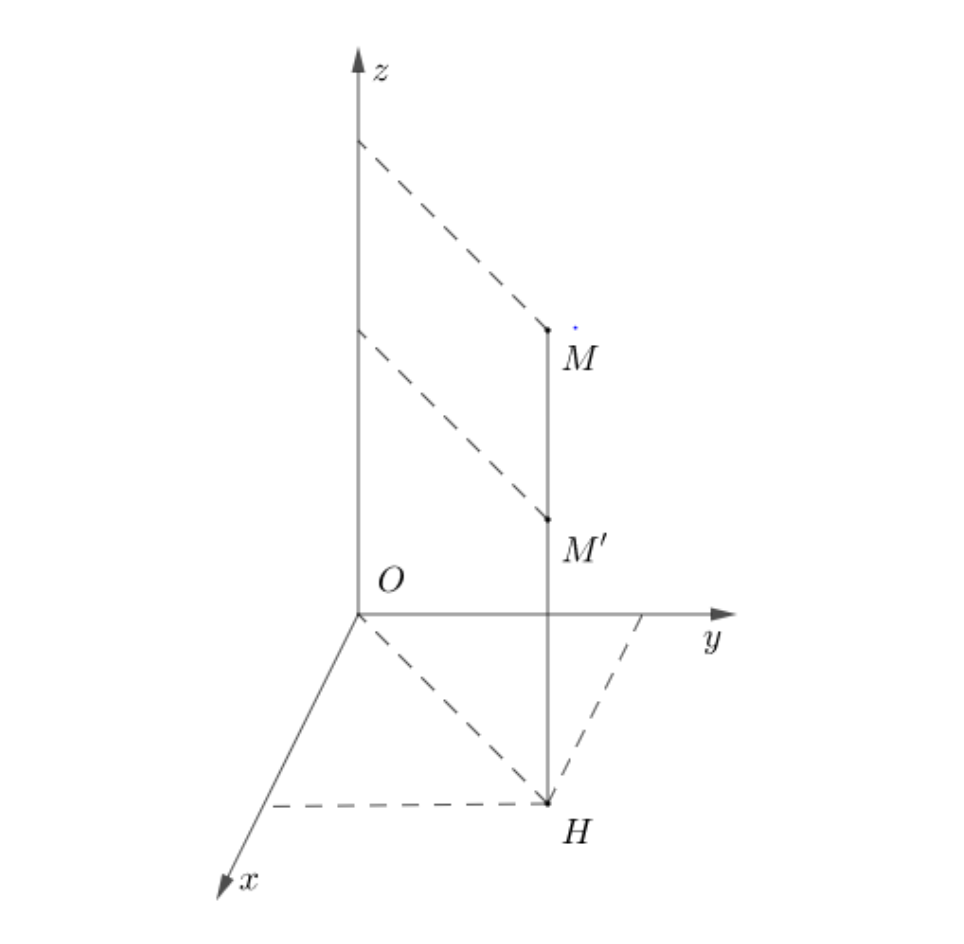
\includegraphics[width=0.5\textwidth]{image/corut.png}
\end{center}
\vspace{0.2cm}
\textbf{5.4.2 Mặt tròn xoay}\\
\vspace{0.2cm}
Điểm $M$ xoay quanh trục $d$ tạo thành đường tròn có tâm là hình chiếu của $M$ lên $d$.\\
Xét điểm $M_0$ có toạ độ $(x_0,y_0,z_0)$ quay quanh trục $Oz$, tạo thành đường tròn $(S)$ có tâm là hình chiếu của $M_0$ lên $Oz$.\\
\begin{center}
    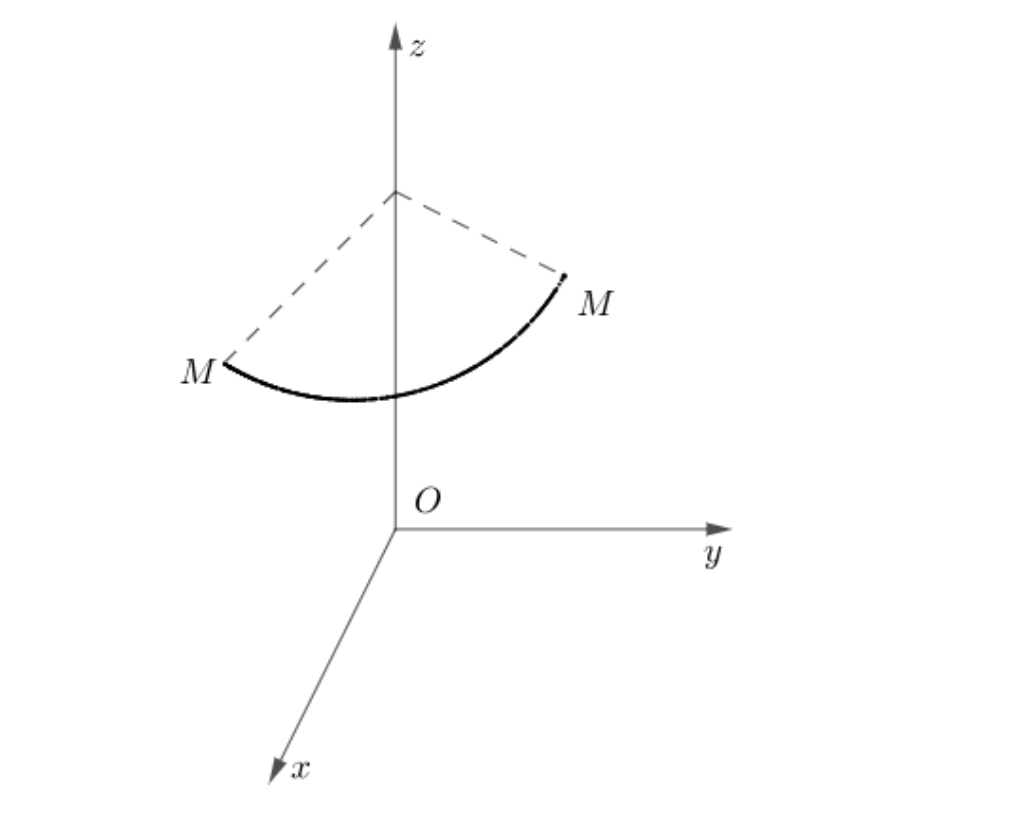
\includegraphics[width=0.5\textwidth]{image/tronxoay.png}
\end{center}
Khi đó, Điểm $M(x,y,z)$ bất kỳ thuộc $(S)$, khi và chỉ khi $d(M,Oz) = d(M_0,Oz)$ và $z = z_0$. Do đó, phương trình của đường tròn $S$ là:
\[
\begin{cases} z = z_0\\x^2 + y^2 = x_0^2 + y_0^2\end{cases}
\]
Cho đường $(C)$ có phương trình $\begin{cases} y = 0\\x = f(z)\end{cases}$ quay xung quanh $Oz$ sẽ tạo thành mặt tròn xoay.\\
Khi đó, $M(x,y,z)$ thuộc mặt tròn xoay khi và chỉ khi tồn tại một điểm $M_0(x_0,y_0,z_0)$ thuộc $C$ sao cho khi $M_0$ quay xung quanh $Oz$ tạo thành đường tròn $(S)$ thì $M \in (S).$\\
$M \in (S)$ khi và chỉ khi $\begin{cases} z = z_0\\x^2 + y^2 = x_0^2 + y_0^2\end{cases}$\\
Mà $M_0 \in (C)$ nên $\begin{cases} y_0 = 0\\x_0 = f(z_0)\end{cases}$\\
Do đó, phương trình của mặt tròn xoay khi quay $(C)$ quanh trục $Oz$ là:\
\[
x^2 + y^2 = f(z)^2
\]
\vspace{0.2cm}
\textbf{5.4.3 Mặt trục và mặt nón}\\
\vspace{0.2cm}
Cho đường $\begin{cases}y = 0 \\ x = a \end{cases}$ quay xung quanh $Oz$ được mặt trong xoay có phương trình:
\[
x^2 + y^2 = f(z)^2
\]
\[
\Leftrightarrow x^2 + y^2 = a^2 \text{   (Mặt trụ tròn xoay)}
\]
\begin{center}
      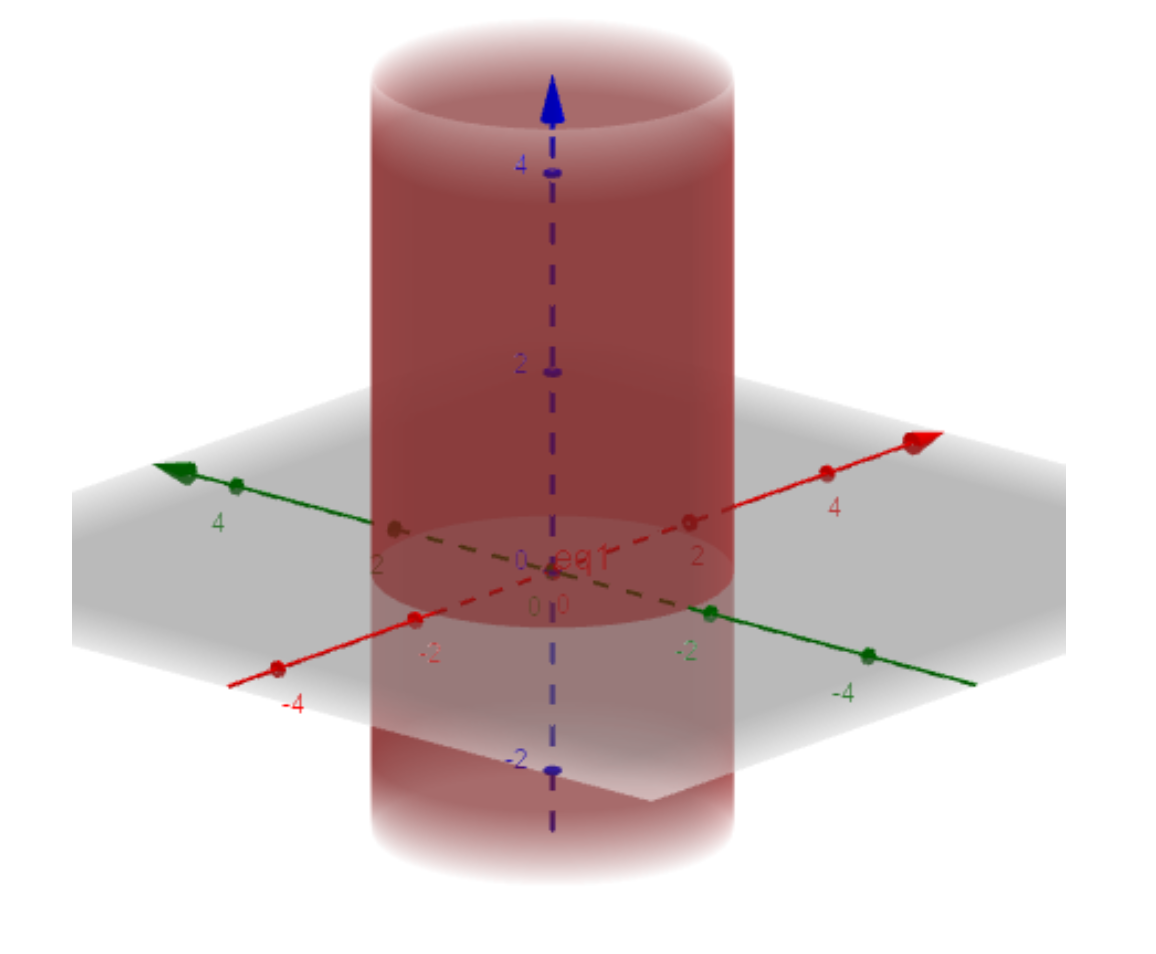
\includegraphics[width=0.5\textwidth]{image/truvanon.png}
\end{center}
Co rút theo phương $Oy$ với tỉ số $\lambda$ ta được mặt trục có phương trình:
\[
\frac{x^2}{a^2} + \frac{y^2}{b^2} = 1
\]
Trong đó $b = \lambda a. $\\
\begin{center}
    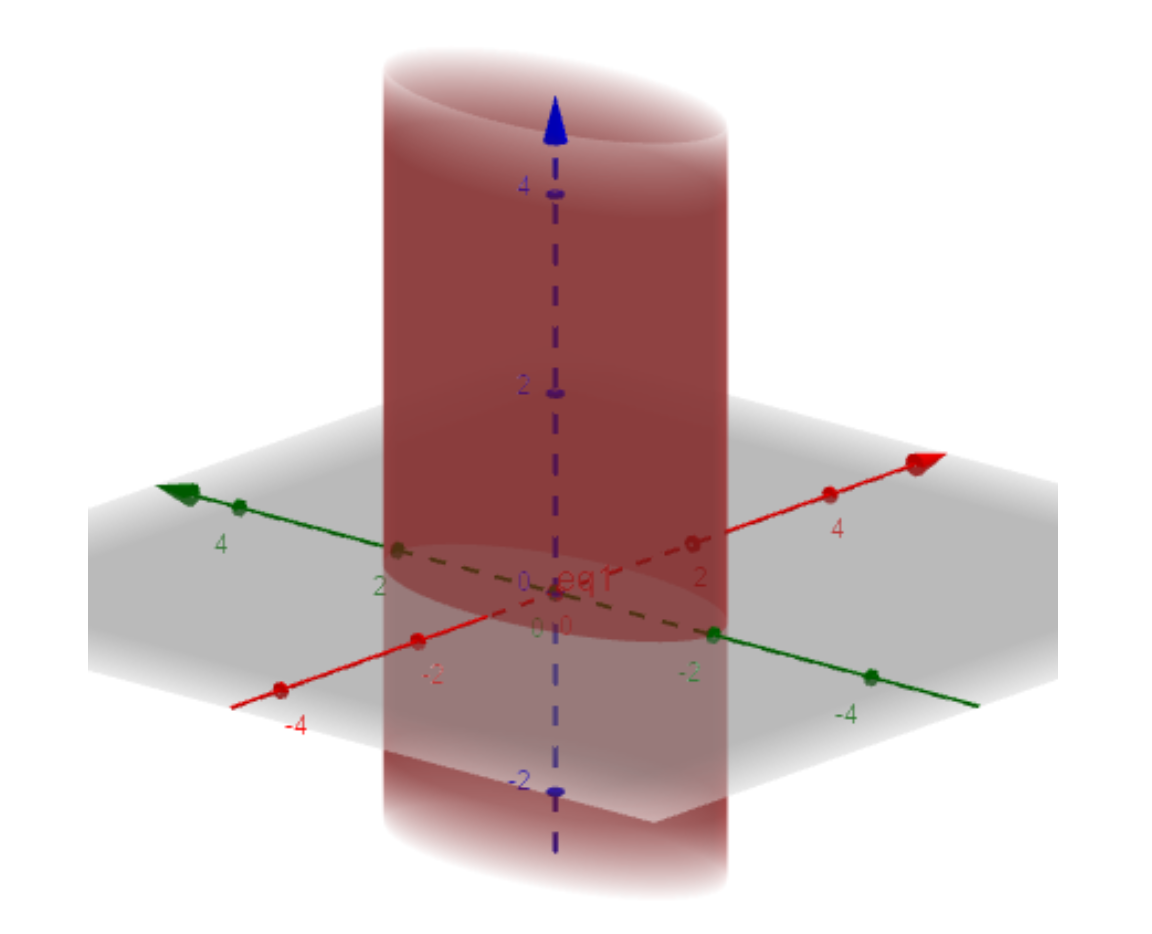
\includegraphics[width=0.5\textwidth]{image/truvanon2.png}
\end{center}
Cho đường thẳng $\begin{cases} y = 0\\x = az\end{cases} (a \neq 0)$quay xung quanh trục $Oz$, ta được mặt tròn xoay có phương trình:
\[
x^2 + y^2 = a^2z^2 \text{ (Mặt nón tròn xoay)}
\]
\begin{center}
    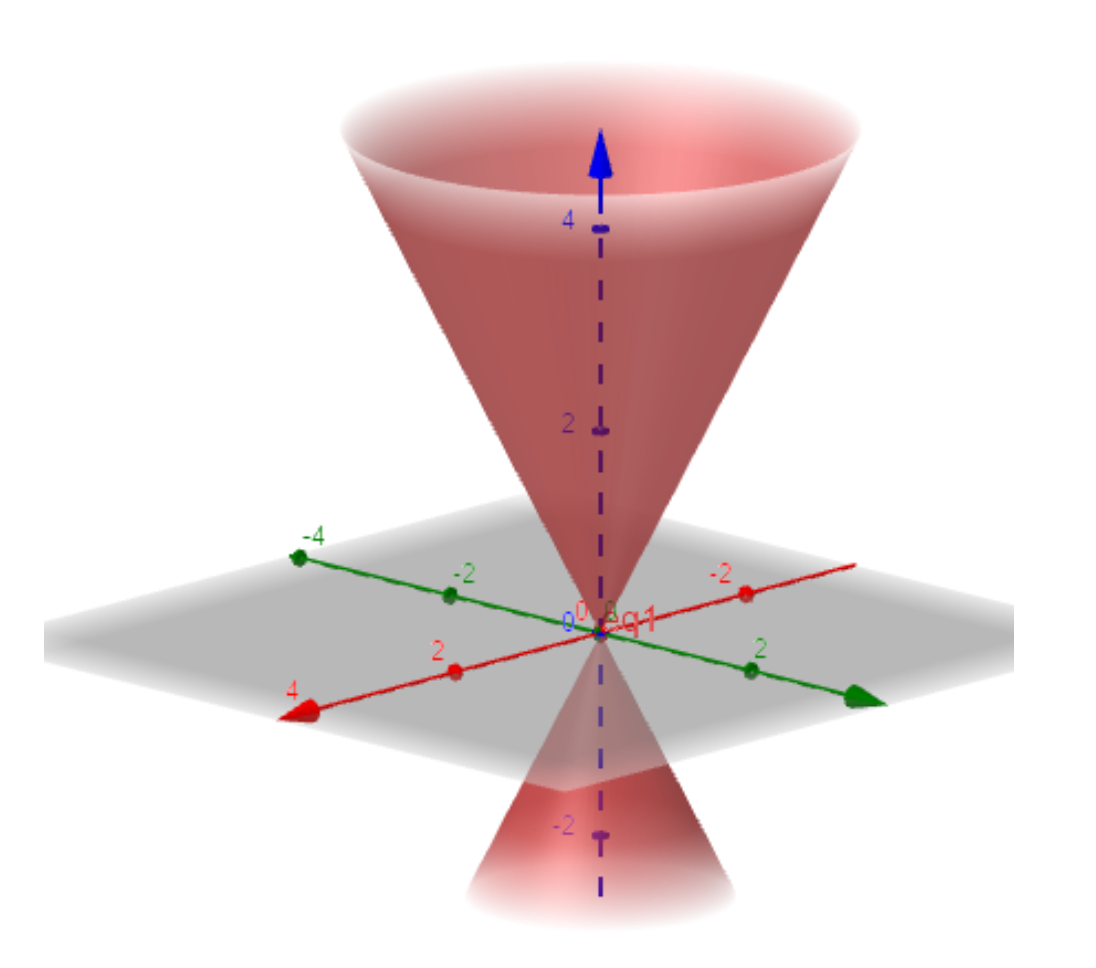
\includegraphics[width=0.5\textwidth]{image/truvanon3.png}
\end{center}
Co rút theo phương $Oy$ với tỉ số $\lambda$ ta được mặt nón có phương trình:
\[
\frac{x^2}{a^2} + \frac{y^2}{b^2} = z^2
\]
Trong đó $b = \lambda a.$\\
\begin{center}
    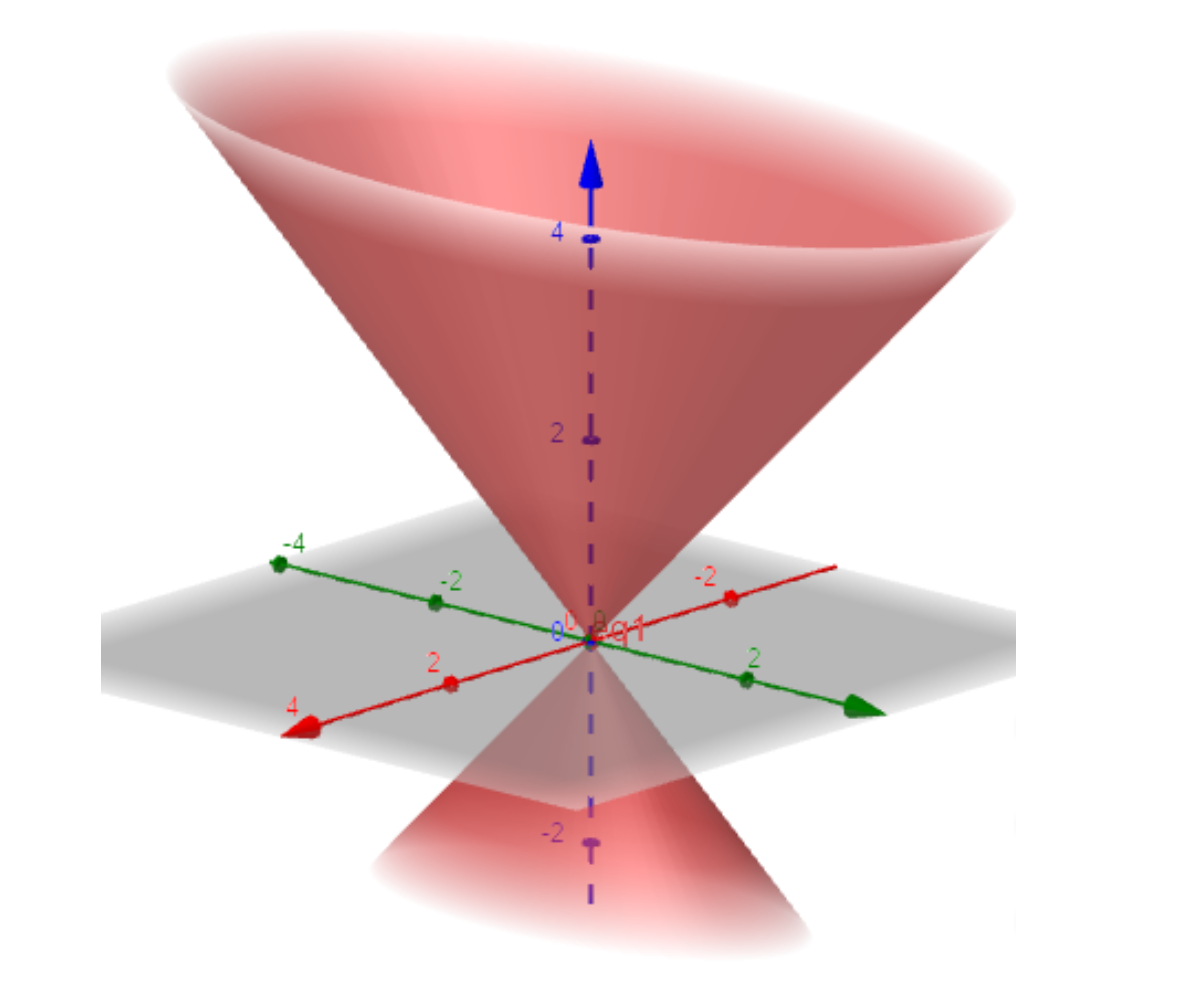
\includegraphics[width=0.5\textwidth]{image/truvanon4.png}
\end{center}
\vspace{0.2cm}
\textbf{5.4.4 Mặt Elipxoit}\\
\vspace{0.2cm}
Cho đường thẳng $\begin{cases} y = 0\\ \frac{x^2}{a^2} + \frac{y^2}{b^2} = 1\end{cases}$ quay xung quanh $Oz$ được mặt tròn xoay có phương trình:
\[
x^2 + y^2 = a^2 (1 - \frac{z^2}{c^2})
\]
\[
\Leftrightarrow \frac{x^2}{a^2} + \frac{y^2}{b^2} + \frac{z^2}{c^2} = 1 \text{ (Elipxoit tròn xoay)}
\]
\begin{center}
    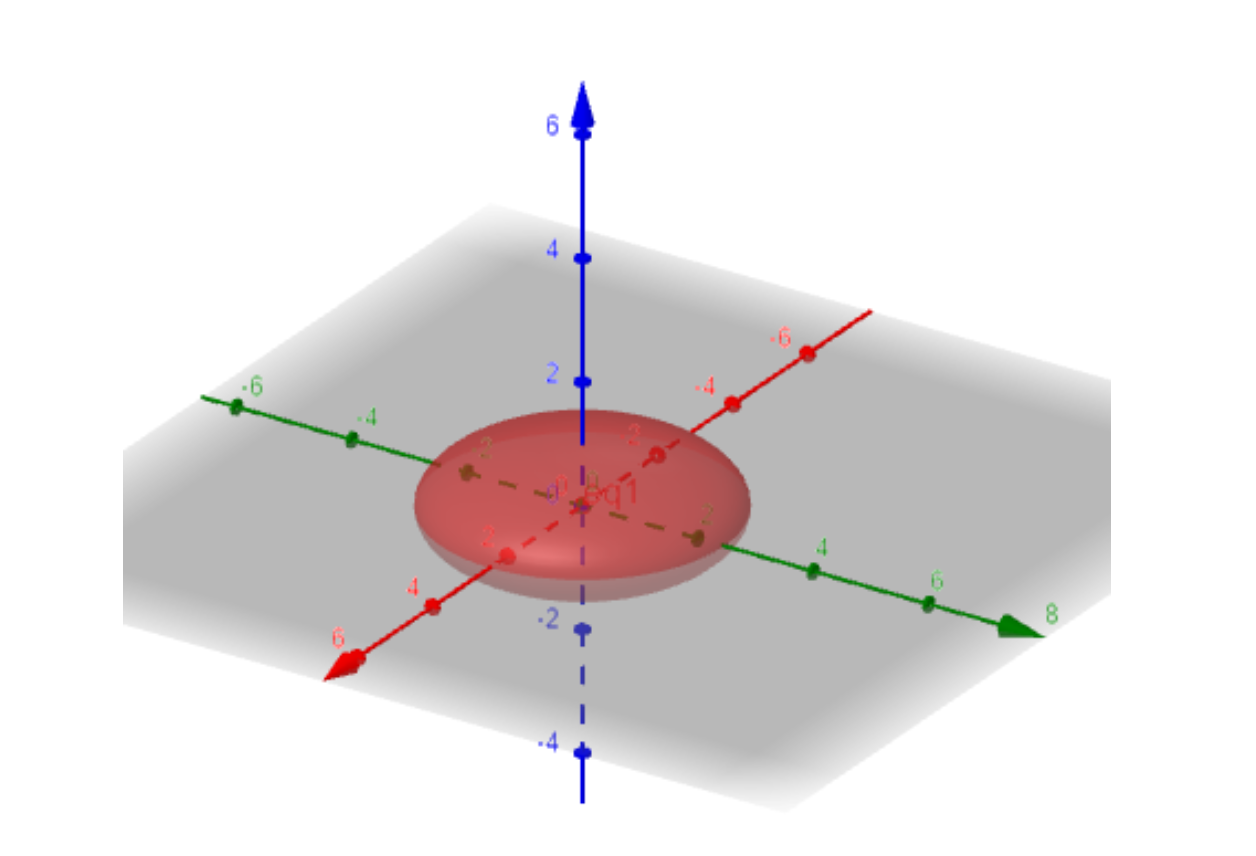
\includegraphics[width=0.5\textwidth]{image/elip.png}
\end{center}
Co rút theo phương $Oy$ với tỉ số $\lambda$ ta được mặt elipxoit có phương trình:
\[
\frac{x^2}{a^2} + \frac{y^2}{b^2} + \frac{z^2}{c^2} = 1
\]
Trong đó $b = \lambda a.$\\
\begin{center}
    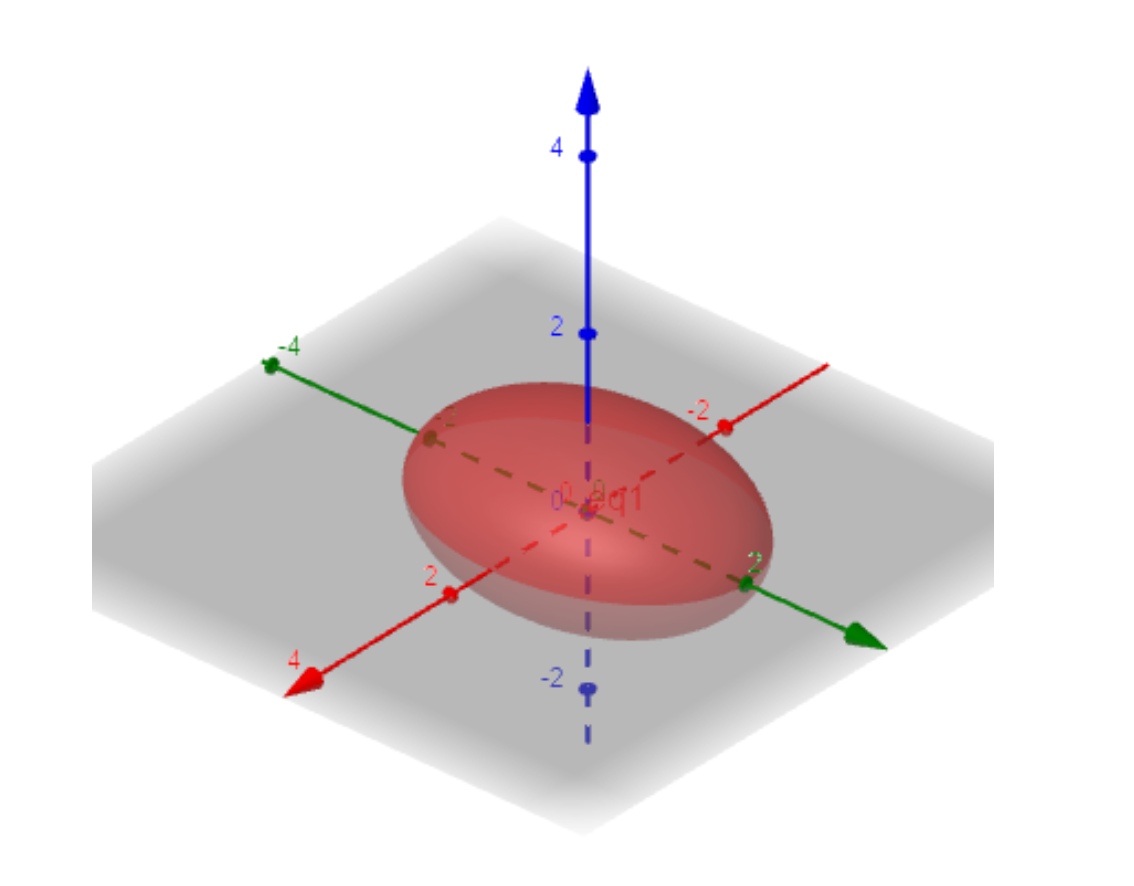
\includegraphics[width=0.5\textwidth]{image/elip2.png}
\end{center}
\vspace{0.2cm}
\textbf{5.4.5 Các mặt Hyperboloit}\\
\vspace{0.2cm}
Cho đường $\begin{cases}y = 0\\\frac{x^2}{a^2} - \frac{z^2}{c^2} = 1\end{cases}$ quay xung quanh $Oz$ được mặt tròn xoay có phương trình:
\[
x^2 + y^2 = f(z)^2
\]
\[
\Leftrightarrow x^2 + y^2 = a^2(1 + \frac{z^2}{c^2})
\]
\[
\Leftrightarrow \frac{x^2}{a^2} + \frac{y^2}{b^2} - \frac{z^2}{c^2} = 1 \text{ (Hyperboloit 1 tầng tròn xoay)}
\]
\begin{center}
    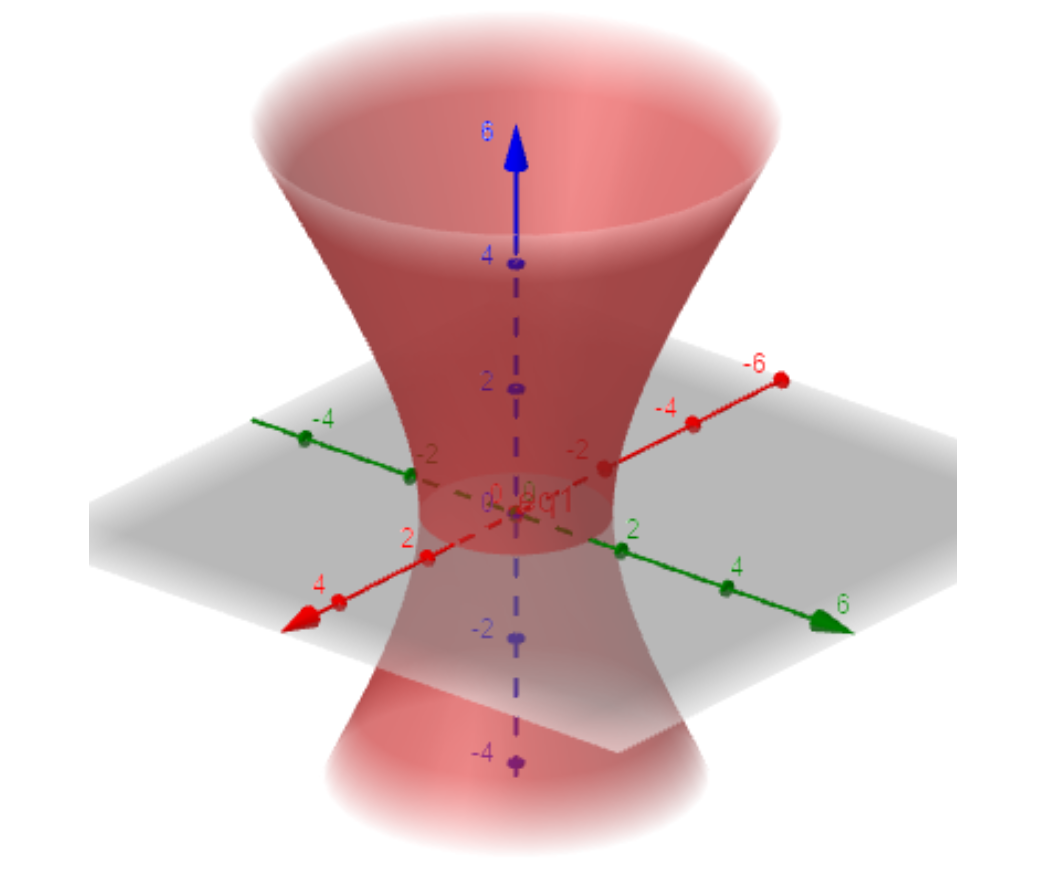
\includegraphics[width=0.5\textwidth]{image/hybepol1.png}
\end{center}
Co rút theo phương $Oy$ với tỉ số $\lambda$ ta được mặt hyperboloit 1 tầng có phương trình:
\[
    \frac{x^2}{a^2} + \frac{y^2}{b^2} - \frac{z^2}{c^2} = 1
\]
Trong đó $b = \lambda a.$\\
\begin{center}
    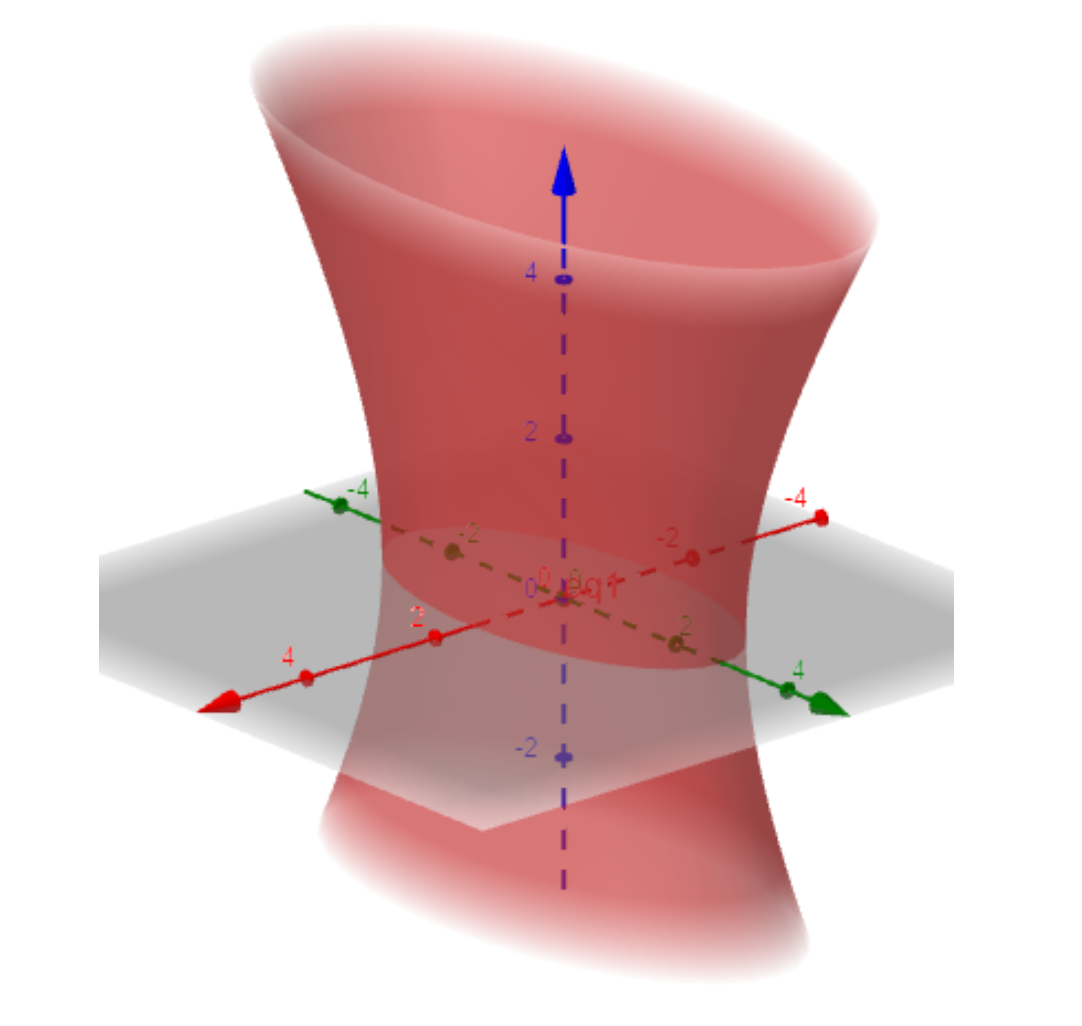
\includegraphics[width=0.5\textwidth]{image/hybepol2.png}
\end{center}
Cho đường $\begin{cases}y = 0\\\frac{x^2}{a^2} - \frac{z^2}{c^2} = 1\end{cases}$ quay xung quanh $Ox$ được mặt tròn xoay có phương trình:
\[
y^2 + z^2 = c^2(\frac{x^2}{a^2} - 1)
\]
\[
\Leftrightarrow \frac{x^2}{a^2} - \frac{y^2}{b^2} - \frac{z^2}{c^2} = 1 \text{ (Hyperboloit 2 tầng tròn xoay)}
\]
\begin{center}
    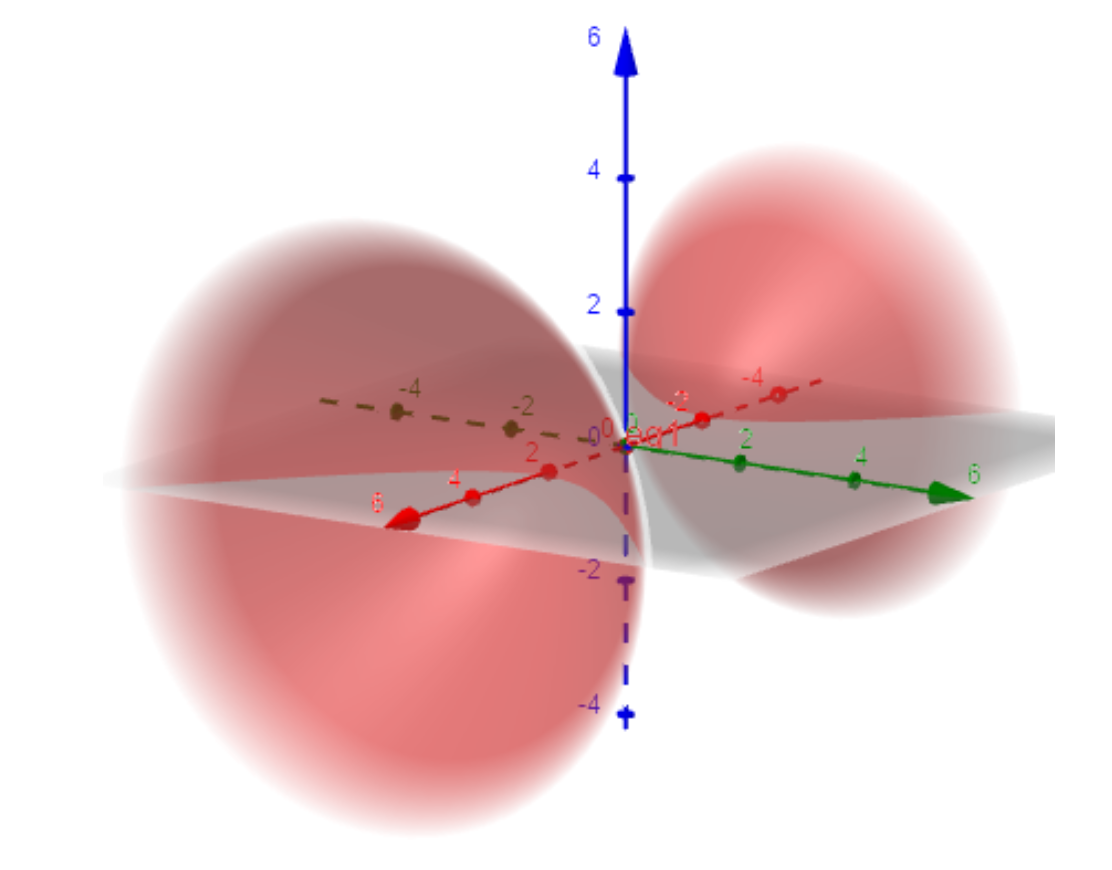
\includegraphics[width=0.5\textwidth]{image/hybepol3.png}
\end{center}
Co rút theo phương $Oy$ với tỉ số $\lambda$ ta được mặt hyperboloit 2 tầng có phương trình:
\[
    \frac{x^2}{a^2} - \frac{y^2}{b^2} - \frac{z^2}{c^2} = 1
\]
Trong đó $b = \lambda a.$\\
\begin{center}
    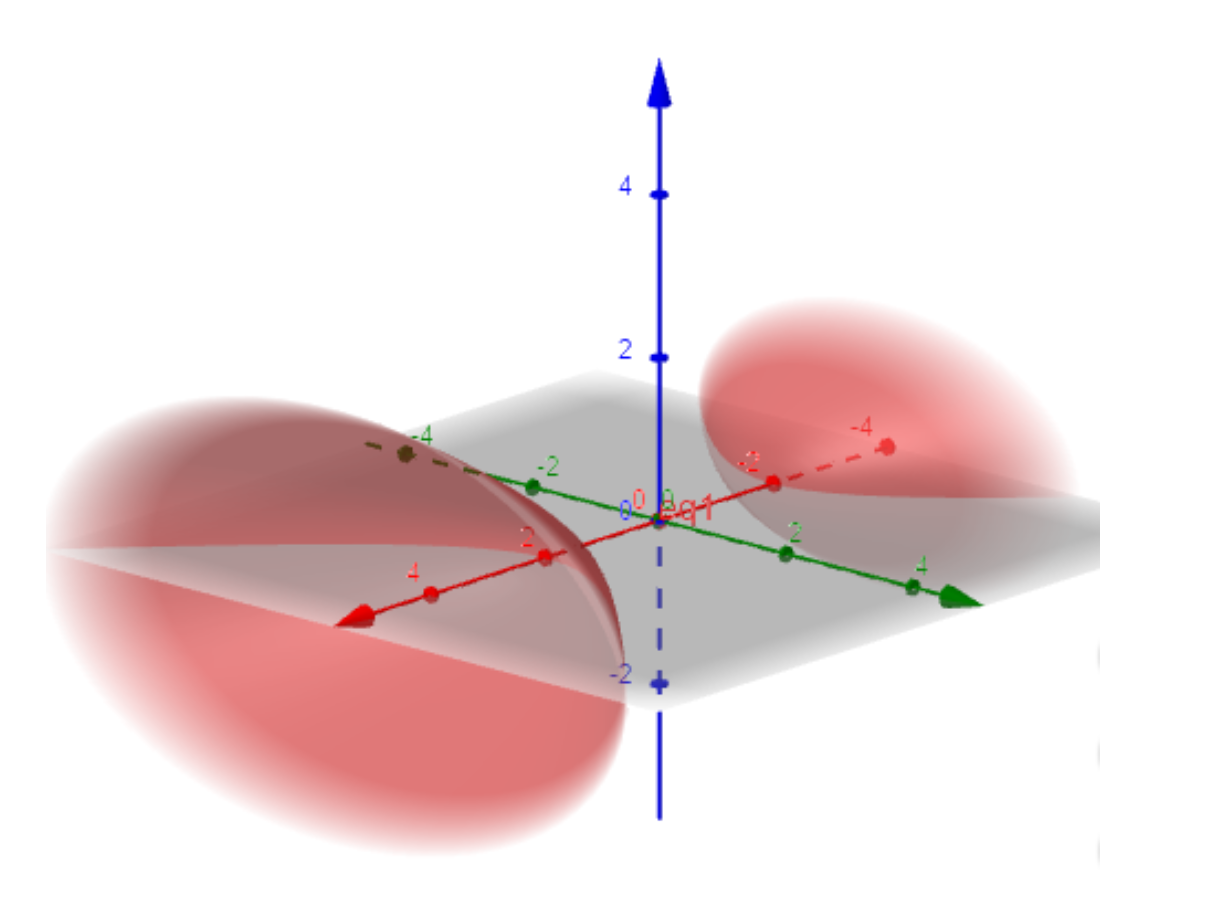
\includegraphics[width=0.5\textwidth]{image/hybepol4.png}
\end{center}
\vspace{0.2cm}
\textbf{5.4.6 Các mặt paraboloit}\\
\vspace{0.2cm}
Cho đường $\begin{cases}y = 0\\x^2 = 2pz \end{cases} (p > 0)$ quay xung quanh $Oz$ được mặt tròn xoay:
\[
x^2 + y^2 = 2pz \text{ (Paraboloit tròn xoay)}
\] 
\begin{center}
    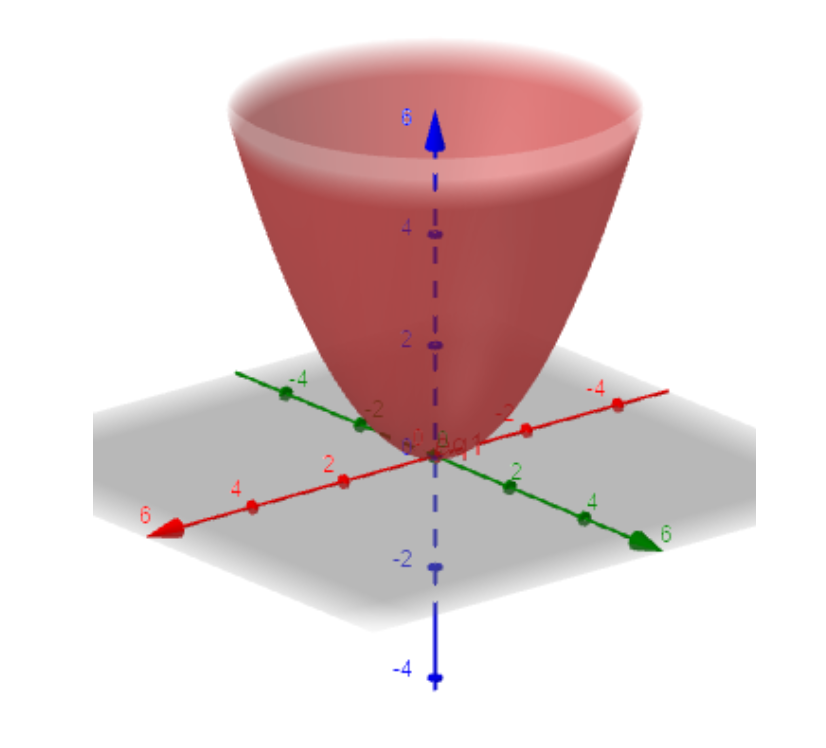
\includegraphics[width=0.5\textwidth]{image/pa1.png}
\end{center}
Co rút theo phương $Oy$ với tỉ số $\lambda$ ta được mặt paraboloit eliptic có phương trình:
\[
\frac{x^2}{a^2} + \frac{y^2}{b^2} = p'z
\]
\begin{center}
    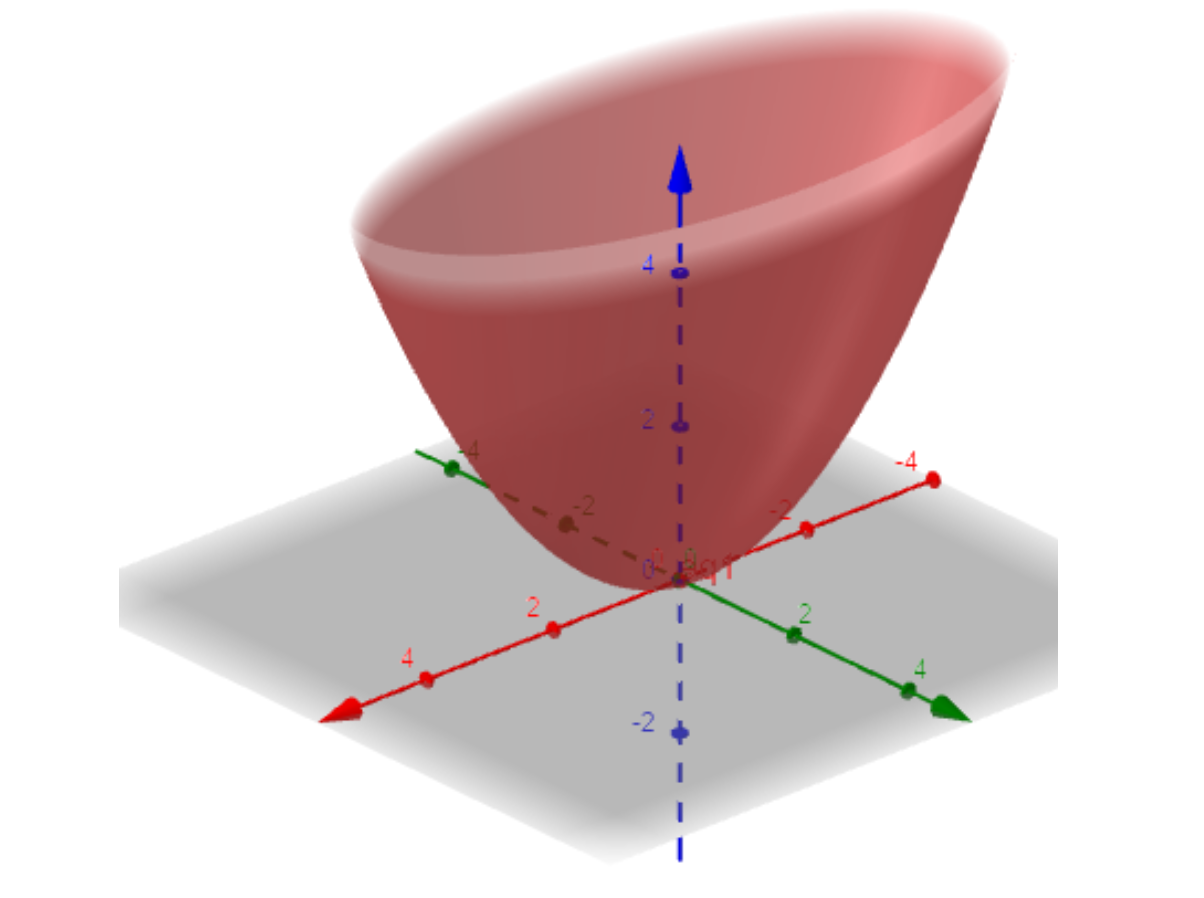
\includegraphics[width=0.5\textwidth]{image/pa2.png}
\end{center}
Mặt có phương trình: $\frac{x^2}{a^2} - \frac{y^2}{b^2} = 2az (p > 0, q > 0)$ được gọi là mặt paraboloit hyperboloic (Mặt yên ngựa).\\
\begin{center}
    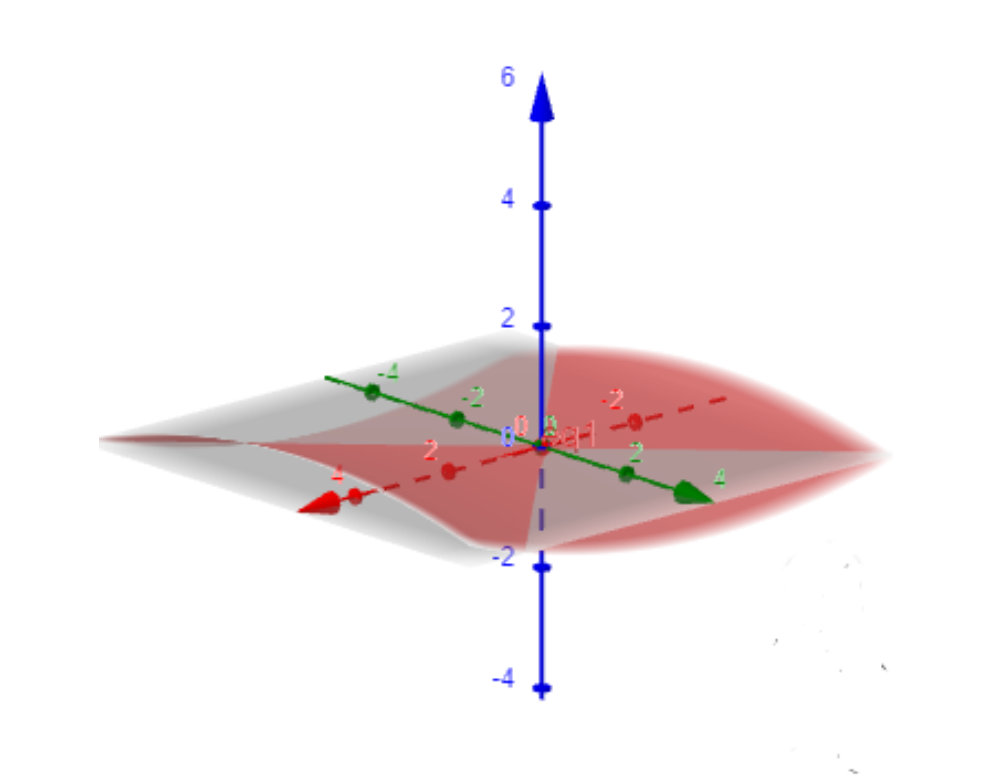
\includegraphics[width=0.5\textwidth]{image/pa3.png}
\end{center}
\textbf{5.5 Mặt kẻ}\\
\textbf{5.5.1 Mặt kẻ}\\
Là mặt mà tại mọi điểm trên mặt đều kẻ được một đường thẳng nằm hoàn toàn trên mặt đó.\\
\vspace{0.2cm}
\textbf{5.5.2 Hyperboloit 1 tầng}\\
\vspace{0.2cm}
Phương trình tổng quát của hyperboloit 1 tầng:
\[
\frac{x^2}{a^2} + \frac{y^2}{b^2} - \frac{z^2}{c^2} = 1
\]
\[
\Leftrightarrow (\frac{x}{a} + \frac{z}{c})(\frac{x}{a} - \frac{z}{c}) = (1 - \frac{y}{b})(1 + \frac{y}{b})
\]
Họ đường thẳng $I: \begin{cases} m(\frac{x}{a} + \frac{z}{c}) = l(1 + \frac{y}{b}) \\ l(\frac{x}{a} - \frac{z}{c}) = m(1 - \frac{y}{b})\end{cases}$\\
Họ đường thẳng $II: \begin{cases} m(\frac{x}{a} + \frac{z}{c}) = l(1 - \frac{y}{b}) \\ l(\frac{x}{a} - \frac{z}{c}) = m(1 + \frac{y}{b})\end{cases}$\\
\vspace{0.2cm}
\textbf{5.5.3 Mặt yên ngựa}\\
\vspace{0.2cm}
Phương trình tổng quát của mặt yên ngựa:
\[
\frac{x^2}{a^2} - \frac{y^2}{b^2} = pz
\]
\[
\Leftrightarrow (\frac{x}{a} + \frac{y}{b})(\frac{x}{a} - \frac{y}{b}) = pz
\]
Họ đường thẳng $I: \begin{cases} m(\frac{x}{a} + \frac{y}{b}) = lp\\l(\frac{x}{a} - \frac{y}{b}) = mz\end{cases}$\\
Họ đường thẳng $II: \begin{cases} m(\frac{x}{a} + \frac{y}{b}) = lz\\l(\frac{x}{a} - \frac{y}{b}) = mp\end{cases}$
\vspace{0.2cm}
\section{Cách chọn mục tiêu}
\vspace{0.2cm}
Dưới đây là một số ví dụ về cách giải toán hình học bằng phương pháp toạ độ và qua đó thấy nên chọn hệ toạ độ như thế nào.\\
\textbf{Ví dụ 1: }Trong mặt phẳng cho hai đường thẳng $(d_1)$ và $(d_2)$ cắt nhau và một điểm $P$ không nằm trên hai đường thẳng đó. Hai đường thẳng phân biệt thay đổi $(d)$ và $(d')$. Qua $P$ và cắt cả $(d_1)$ và $(d_2)$. Ta gọi $A = (d) \cap (d_1), B = (d) \cap (d_2). A' = (d') \cap (d_1), B' = (d') \cap (d_2).$ Tìm quỹ tích giao điểm $M$ của hai đường thẳng $AB' \text{ và } A'B$.\\
\textbf{Hướng dẫn giải}\\
Gọi $O$ là giao điểm của $d_1$ và $d_2$. Lấy hai điểm $I$ và $J$ lần lượt nằm trên $d_1$ và $d_2$ sao cho $\overrightarrow{OP} = \overrightarrow{OI} + \overrightarrow{OJ}$ và đặt $\overrightarrow{OI} = \vec{i}, \overrightarrow{OJ} = \vec{j}.$\\
Ta chọn mục tiêu affine là $(O; \vec{i}; \vec{j}).$ Khi đó điểm $P$ có toạ độ $(1; 1).$ Giả sử các giao điểm có toạ độ là $A = (a, 0), B = (0, b), A' = (a', 0), B' = (0, b').$ Khi đó đường thẳng $(d)$ có phương trình $\frac{x}{a} + \frac{y}{b} = 1,$ mà $(d)$ cũng đi qua $P(1,1)$ nên ta có:
\[
\frac{1}{a} + \frac{1}{b} = 1 \text{ }(1).
\]
Tương tự có:
\[
    \frac{1}{a'} + \frac{1}{b'} = 1 \text{ }(2).
\]
Các đường thẳng $AB'$ và $A'B$ lần lượt có phương trình:
\[
\frac{x}{a} + \frac{y}{b'} = 1 \text{ }(3) \hspace{0.5cm} \text{ và } \frac{x}{a'} + \frac{y}{b} = 1 \text{ }(4).
\]
\begin{center}
    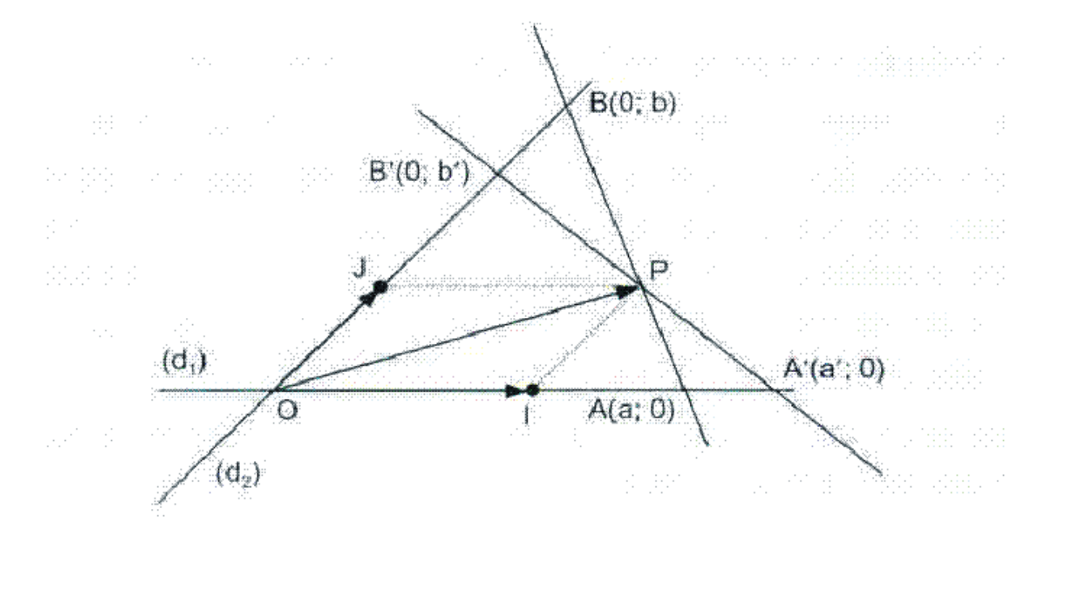
\includegraphics[width=0.5\textwidth]{image/bt1.png}
\end{center}
Điểm $M$ là giao điểm của $AB'$ và $A'B$ khi và chỉ khi nó có toạ độ $(x,y)$ thoả mãn cả hai phương trình $(3), (4)$, suy ra nó thoả mãn phương trình sau đây (bằng cách trừ hai phương trình đó):
\[
(\frac{1}{a} - \frac{1}{a'})x + (\frac{1}{b'} - \frac{1}{b})y = 0 \text{ }(5).
\]
Chú ý rằng, từ hai điều kiện $(1)$ và $(2)$ ta suy ra (bằng cách trừ hai đẳng thức đó):
\[
\frac{1}{a} - \frac{1}{a'} = \frac{1}{b'} - \frac{1}{b}
\]
Từ $(5)$ trở thành: $x + y = 0.$ Vậy điểm $M$ thuộc đường thẳng $(\Delta)$ có phương trình: $x + y = 0.$\\
Ngược lại, giả sử $M_0(x_0,y_0)$ là một điểm trên đường thẳng $(\Delta)$ và $M_0 \neq 0.$ Ta lấy một số a tuỳ ý khác 0 và 1m rồi xác định các số b, a', b' sao cho:
\[
\frac{1}{a} + \frac{1}{b} = 1, \frac{1}{a'} - \frac{1}{b} = \frac{1}{x_0}, \frac{1}{a} - \frac{1}{b'} = \frac{1}{x_0}.
\]
Khi đó ta cũng có $\frac{1}{a'} + \frac{1}{b'} = 1.$\\
Gọi $A = (a,0), A' = (a',0), B = (0,b), B' = (0,b').$ Gọi $(d_1)$ và $(d_2)$ lần lượt là các đường thẳng $AB$ và $A'B'$ thì phương trình $(d_1)$ và $(d_2)$ lần lượt là:
\[
\frac{x}{a} + \frac{y}{b} = 1 \text{ và } \frac{x}{a'} + \frac{y}{b'} = 1.
\]
Điều đó chứng tỏ $(d_1)$ và $(d_2)$ đều đi qua $P(1,1)$. Các đường thẳng $AB'$ và $B'A$ có phương trình lần lượt là $\frac{x}{a} + \frac{y}{b'} = 1$ và $\frac{x}{a'} + \frac{y}{b} = 1.$ Thay toạ độ $(x_0,-x_0)$ của điểm $M_0$ vào cả hai phương trình ta suy ra $AB'$ và $B'A$ cắt nhau tại $M_0$. Tóm lại quỹ tích của $M$ là đường thẳng $x + y = 0.$\\
\textbf{Chú ý:} Đối với bài toán này nếu dùng hệ toạ độ trực chuẩn thì rất phức tạp. Nếu dùng toạ độ affine thì hiển nhiên nên chọn các đường thẳng $(d_1)$ và $(d_2)$ làm trục toạ độ và $O$ là gốc toạ độ. Khi đó $P$ có toạ độ $(x_0,y_0)$. Vì giả thiết cho điểm $P$ không nằm trên $(d_1)$ và $(d_2)$ nên ta có thể chọn các vector cơ sở của hệ toạ độ sao cho $P$ có toạ độ $(1,1)$ để các phép tính được đơn giản hơn.\\
\vspace{0.2cm}
\textbf{Ví dụ 2:} Trong mặt phẳng cho hai đường thẳng cắt nhau $a$ và $b$. Tìm quỹ tích những điểm M sao cho tích các khoảng cách từ M tới a và b bằng một số không đổi $k^2 \neq 0.$\\
\begin{center}
    \begin{tikzpicture}[scale=1.5]

        % Vẽ các trục tọa độ
        \draw[->,thick] (0,0) -- (3,0) node[anchor=north] {$x$}; % Trục x
        \draw[->,thick] (0,0) -- (0,3) node[anchor=west] {$y$}; % Trục y
    
        
        % Vẽ các vector
        \draw[->,thick] (0,0) -- (2,0.7) node[anchor=west] {$a$}; % Vector a
        \draw[->,thick] (0,0) -- (2,-0.7) node[anchor=west] {$b$}; % Vector b
        
        % Đánh dấu gốc tọa độ
        \filldraw (0,0) circle (1pt) node[anchor=north east] {$O$};
        
        \end{tikzpicture}
\end{center}
\textbf{Hướng dẫn giải}\\
Bài toán liên quan tới khoảng cách nên ta không dừng hệ toạ độ affine mà phải dùng hệ toạ độ trực chuẩn. Do tính đối xứng của các cặp đường thẳng cắt nhau ta sẽ chọn hệ toạ độ trực chuẩn $Oxy$ sao cho $Ox$ và $Oy$ là hai đường phân giác của các góc hợp bởi hai đường thẳng $a$ và $b$.\\
Khi đó phương trình đường thẳng $a$ và $b$ lần lượt là:
\[
x + py = 0 \text{ và } x - py = 0.
\]
Nếu $M = (x,y)$ thì khoảng cách từ $M$ tới $a$ và $b$ lần lượt là:
\[
d = d(M,(a)) = \frac{|x + py|}{\sqrt{1 + p^2}}; d' = d(M,(b)) = \frac{|x - py|}{\sqrt{1 + p^2}}.
\]
Vậy ta tìm quỹ tích các điểm $M$ sao cho $d\cdot d' = d(M,(a)) \cdot d(M,(b)) = k^2$, thoả mãn:
\[
\frac{|x + py|}{\sqrt{1 + p^2}} \cdot \frac{|x - py|}{\sqrt{1 + p^2}} = k^2 \Leftrightarrow \frac{|x^2 - p^2y^2|}{1 + p^2} = k^2.
\]
\[
\Leftrightarrow x^2 - p^2y^2 = \pm k^2(1 + p^2).
\]
Vậy quỹ tích các điểm $M$ là hai đường hypebol.
\vspace{0.2cm}
\section{Các dạng bài tập}
\vspace{0.2cm}
\textbf{Bài toán 1:} Cho đường thẳng $d$ và điểm $p$ nằm ngoài $d$. Tìm quỹ tích những điểm $M$ cách đều $p$ và $d$.\\
Bài toán này là một phát triển rất tự nhiên của hai quỹ tích quen thuộc: Quỹ tích những điểm cách đều 2 điểm đã cho là một đường trung trực của đoạn thẳng nối hai điểm này, quỹ tích những điểm cách đều hai đường thẳng đã cho là các đường phân giác của một góc tạo bởi hai đường thẳng này.\\
Vậy quỹ tích những điểm cách đều một điểm đã cho và một đường thẳng đã cho là gì?\\
Phân tích một số vị trí đặc biệt, có thể thấy quỹ tích không phải là đường thẳng mà cũng không phải là đường tròn (chẳng hạn trung điểm đoạn vuông góc PH thuộc quỹ tích và tập quỹ tích đối xứng qua đường thằng PH). Vậy quỹ tích có thể là gì? Ta hãy đưa hệ trục toạ độ vào. Một cách tự nhiên, ta chọn HP là trục tung và d là trục hoành. Đặt HP = p thì $P(0,p)$. Giả sử $M(x,y)$ là một điểm thuộc quỹ tích thì rõ ràng $V > 0$ và ta có:
\[
MP = d(M,d) \Leftrightarrow \sqrt{x^2 + (y - p)^2} = y \Leftrightarrow x^2 + (y - p)^2 = y^2
\]
\[
\Leftrightarrow x^2 - 2py + p^2 = 0 \Leftrightarrow y = \frac{1}{2p}x^2 + \frac{p}{2}.
\]
Quỹ tích là một parabol.\\
Đây cũng chính là một thế mạnh của hình học giải tích so với hình học thuần tuý.\\
Hình học giải tích cho phép tìm ra các quỹ tích vượt ngoài ra các hình vẽ được bằng thước và compa, nghiên cứu các tính chất hình học của các đường cong đại số bất kỳ.\\
\textbf{Bài toán 2:} Cho tam giác ABC cân tại A. M là một điểm bất kỳ nằm trong tam giác. Chứng minh rằng $MA^2 + MB\cdot MC \leq AB^2.$\\
Hạ đường cao AH và chọn hệ trục toạ độ lấy $H$ làm gốc toạ độ, BC và HA là các trục toạ độ. Đặt $B(-b,0), C(b,0) và A(0,a).$ Với điểm $M(x,y),$ bất đẳng thức cần chứng minh tương đường với:
\[
\Leftrightarrow x^2 + (y - a)^2 + \sqrt{(x + b)^2 + y^2} \cdot \sqrt{(x - b)^2 + y^2} \leq a^2 + b^2
\]
\[
\Leftrightarrow \sqrt{(x^2 + y^2 + b^2)^2 -  4b^2x^2} \leq b^2 - x^2 - y^2 + 2ay
\]
\[
\Leftrightarrow (x^2 + y^2 + b^2)^2 - 4b^2x^2 \leq (b^2 - x^2 -y^2)^2 + 4ay(b^2 - x^2 - y^2) + 4a^2y^2
\]
\[
\Leftrightarrow b^2y^2 \leq ay(b^2 - x^2 - y^2) + a^2y^2
\]
Bất đẳng thức này trở thành đẳng thức khi $y = 0.$ với $y > 0.$ Bất đẳng thức này tương đương với:
\[
ax^2 \leq (a^2 - b^2)y + a(b^2 - y^2) \hspace{0.5cm} (3)
\]
Dữ kiện $M$ nằm trong tam giác ABC bây giờ cho ta:
\[
|x| \leq (\frac{b}{a})(a - y)
\]
Thay vào (3), ta cần chứng minh:
\[
b^2(a - y)^2 \leq a(a^2 - b^2)y + a^2(b^2 - y^2)
\]
Sau các phép rút gọnm điều này tương đương với
\[
y^2 \leq ay
\]
Nhưng điều này đúng vì $0 < y \leq a.$
\section{Bài tập làm thêm}
\textbf{Bài toán 1:} (Công thức tính độ dài trung tuyến) Cho tam giác ABC có độ dài các cạnh BC, CA, AB lần lượt là a, b, c. Chứng minh rằng độ dài trung tuyến AM có thể tính theo công thức
\[
m_a^2 = \frac{(2b^2 + 2c^2 - a^2)}{4}
\]
\textbf{Bài toán 2:} Cho hình vuông ABCD cạnh bằng 1. Hai điểm M, N di chuyển trên BC, CD tương ứng sao cho chu vi tam giác CMN bằng 2. Chứng minh $\angle MAN = 45 \degree. $\\
\textbf{Bài toán 3:} Cho tam giác đều ABC. M là một điểm bất kỳ trong mặt phẳng tam giác. Gọi D, E, F là chân các đường vuông góc hạ từ M xuống BC, CA, AB. Chứng minh rằng\
\[
P = MA^2 + MB^2 + MC^2 - 2(MD^2 + ME^2 + MF^2)
\]
Là một đại lượng không đổi.\\
\textbf{Bài toán 4:} (Hệ thức Euler) Cho tam giác ABC có tâm đường tròn ngoại tiếp $O$ và tâm đường tròn nội tiếp $I$. Chứng minh hệ thức
\[
IO^2 = R^2 - 2Rr
\]
\textbf{Bài toán 5:} (Đường thẳng Euler) Chứng minh rằng trong tam giác ABC bất kỳ, trọng tâm, trực tâm và tâm đường tròn ngoại tiếp nằm trên một đường thẳng.
\section{Tài liệu tham khảo}
$[1]$. Phương pháp toạ độ trên mặt phẳng.\\
$[2]$. Phương pháp toạ độ trong không gian.\\
$[3]$. Giáo trình hình học giải tích - Văn Như Cường.\\
$[4]$. Phương pháp toạ độ - Toán cao cấp c1 - Đại học Sài Gòn.\\
\end{titlepage}
\end{document}
